% Options for packages loaded elsewhere
\PassOptionsToPackage{unicode}{hyperref}
\PassOptionsToPackage{hyphens}{url}
\PassOptionsToPackage{dvipsnames,svgnames,x11names}{xcolor}
%
\documentclass[
  12pt,
  a4paper,
  extrafontsizes,
  onecolumn,
  openright]{memoir}

\usepackage{amsmath,amssymb}
\usepackage{iftex}
\ifPDFTeX
  \usepackage[T1]{fontenc}
  \usepackage[utf8]{inputenc}
  \usepackage{textcomp} % provide euro and other symbols
\else % if luatex or xetex
  \usepackage{unicode-math}
  \defaultfontfeatures{Scale=MatchLowercase}
  \defaultfontfeatures[\rmfamily]{Ligatures=TeX,Scale=1}
\fi
\usepackage{lmodern}
\ifPDFTeX\else  
    % xetex/luatex font selection
  \setmainfont[Extension=.otf,UprightFont=*-regular,BoldFont=*-bold,BoldItalicFont=*-bolditalic,ItalicFont=*-italic]{texgyretermes}
  \setmathfont[]{texgyretermes-math.otf}
\fi
% Use upquote if available, for straight quotes in verbatim environments
\IfFileExists{upquote.sty}{\usepackage{upquote}}{}
\IfFileExists{microtype.sty}{% use microtype if available
  \usepackage[]{microtype}
  \UseMicrotypeSet[protrusion]{basicmath} % disable protrusion for tt fonts
}{}
\makeatletter
\@ifundefined{KOMAClassName}{% if non-KOMA class
  \IfFileExists{parskip.sty}{%
    \usepackage{parskip}
  }{% else
    \setlength{\parindent}{0pt}
    \setlength{\parskip}{6pt plus 2pt minus 1pt}}
}{% if KOMA class
  \KOMAoptions{parskip=half}}
\makeatother
\usepackage{xcolor}
\setlength{\emergencystretch}{3em} % prevent overfull lines
\setcounter{secnumdepth}{5}
% Make \paragraph and \subparagraph free-standing
\ifx\paragraph\undefined\else
  \let\oldparagraph\paragraph
  \renewcommand{\paragraph}[1]{\oldparagraph{#1}\mbox{}}
\fi
\ifx\subparagraph\undefined\else
  \let\oldsubparagraph\subparagraph
  \renewcommand{\subparagraph}[1]{\oldsubparagraph{#1}\mbox{}}
\fi
% pandoc tempate
%%%%%%%%%%%%%%%%%%%%%%%%%%%%%%%%%%%%%%%%%%%%%%%%%%%%%%%%%%

\usepackage{color}
\usepackage{fancyvrb}
\newcommand{\VerbBar}{|}
\newcommand{\VERB}{\Verb[commandchars=\\\{\}]}
\DefineVerbatimEnvironment{Highlighting}{Verbatim}{commandchars=\\\{\}}
% Add ',fontsize=\small' for more characters per line
\usepackage{framed}
\definecolor{shadecolor}{RGB}{241,243,245}
\newenvironment{Shaded}{\begin{snugshade}}{\end{snugshade}}
\newcommand{\AlertTok}[1]{\textcolor[rgb]{0.68,0.00,0.00}{#1}}
\newcommand{\AnnotationTok}[1]{\textcolor[rgb]{0.37,0.37,0.37}{#1}}
\newcommand{\AttributeTok}[1]{\textcolor[rgb]{0.40,0.45,0.13}{#1}}
\newcommand{\BaseNTok}[1]{\textcolor[rgb]{0.68,0.00,0.00}{#1}}
\newcommand{\BuiltInTok}[1]{\textcolor[rgb]{0.00,0.23,0.31}{#1}}
\newcommand{\CharTok}[1]{\textcolor[rgb]{0.13,0.47,0.30}{#1}}
\newcommand{\CommentTok}[1]{\textcolor[rgb]{0.37,0.37,0.37}{#1}}
\newcommand{\CommentVarTok}[1]{\textcolor[rgb]{0.37,0.37,0.37}{\textit{#1}}}
\newcommand{\ConstantTok}[1]{\textcolor[rgb]{0.56,0.35,0.01}{#1}}
\newcommand{\ControlFlowTok}[1]{\textcolor[rgb]{0.00,0.23,0.31}{#1}}
\newcommand{\DataTypeTok}[1]{\textcolor[rgb]{0.68,0.00,0.00}{#1}}
\newcommand{\DecValTok}[1]{\textcolor[rgb]{0.68,0.00,0.00}{#1}}
\newcommand{\DocumentationTok}[1]{\textcolor[rgb]{0.37,0.37,0.37}{\textit{#1}}}
\newcommand{\ErrorTok}[1]{\textcolor[rgb]{0.68,0.00,0.00}{#1}}
\newcommand{\ExtensionTok}[1]{\textcolor[rgb]{0.00,0.23,0.31}{#1}}
\newcommand{\FloatTok}[1]{\textcolor[rgb]{0.68,0.00,0.00}{#1}}
\newcommand{\FunctionTok}[1]{\textcolor[rgb]{0.28,0.35,0.67}{#1}}
\newcommand{\ImportTok}[1]{\textcolor[rgb]{0.00,0.46,0.62}{#1}}
\newcommand{\InformationTok}[1]{\textcolor[rgb]{0.37,0.37,0.37}{#1}}
\newcommand{\KeywordTok}[1]{\textcolor[rgb]{0.00,0.23,0.31}{#1}}
\newcommand{\NormalTok}[1]{\textcolor[rgb]{0.00,0.23,0.31}{#1}}
\newcommand{\OperatorTok}[1]{\textcolor[rgb]{0.37,0.37,0.37}{#1}}
\newcommand{\OtherTok}[1]{\textcolor[rgb]{0.00,0.23,0.31}{#1}}
\newcommand{\PreprocessorTok}[1]{\textcolor[rgb]{0.68,0.00,0.00}{#1}}
\newcommand{\RegionMarkerTok}[1]{\textcolor[rgb]{0.00,0.23,0.31}{#1}}
\newcommand{\SpecialCharTok}[1]{\textcolor[rgb]{0.37,0.37,0.37}{#1}}
\newcommand{\SpecialStringTok}[1]{\textcolor[rgb]{0.13,0.47,0.30}{#1}}
\newcommand{\StringTok}[1]{\textcolor[rgb]{0.13,0.47,0.30}{#1}}
\newcommand{\VariableTok}[1]{\textcolor[rgb]{0.07,0.07,0.07}{#1}}
\newcommand{\VerbatimStringTok}[1]{\textcolor[rgb]{0.13,0.47,0.30}{#1}}
\newcommand{\WarningTok}[1]{\textcolor[rgb]{0.37,0.37,0.37}{\textit{#1}}}

\providecommand{\tightlist}{%
  \setlength{\itemsep}{0pt}\setlength{\parskip}{0pt}}\usepackage{longtable,booktabs,array}
\usepackage{calc} % for calculating minipage widths
% Correct order of tables after \paragraph or \subparagraph
\usepackage{etoolbox}
\makeatletter
\patchcmd\longtable{\par}{\if@noskipsec\mbox{}\fi\par}{}{}
\makeatother
% Allow footnotes in longtable head/foot
\IfFileExists{footnotehyper.sty}{\usepackage{footnotehyper}}{\usepackage{footnote}}
\makesavenoteenv{longtable}
\usepackage{graphicx}
\makeatletter
\def\maxwidth{\ifdim\Gin@nat@width>\linewidth\linewidth\else\Gin@nat@width\fi}
\def\maxheight{\ifdim\Gin@nat@height>\textheight\textheight\else\Gin@nat@height\fi}
\makeatother
% Scale images if necessary, so that they will not overflow the page
% margins by default, and it is still possible to overwrite the defaults
% using explicit options in \includegraphics[width, height, ...]{}
\setkeys{Gin}{width=\maxwidth,height=\maxheight,keepaspectratio}
% Set default figure placement to htbp
\makeatletter
\def\fps@figure{htbp}
\makeatother

% Add LaTeX code into the preamble of the document here
\hyphenation{bio-di-ver-si-ty sap-lings}

% Define colors for text boxes
\definecolor{grey}{HTML}{F5F5F5}

% Define text box environments
\usepackage[tikz]{bclogo}
\newmdenv[
  style=boxstyle,
  backgroundcolor=grey,
  frametitlebackgroundcolor=grey,
]{greybox}

\usepackage[automake]{glossaries-extra}
\makeglossaries


\usepackage{amsmath}
\usepackage{booktabs}
\usepackage{caption}
\usepackage{longtable}
\makeatletter
\makeatother
\makeatletter
\@ifpackageloaded{bookmark}{}{\usepackage{bookmark}}
\makeatother
\makeatletter
\@ifpackageloaded{caption}{}{\usepackage{caption}}
\AtBeginDocument{%
\ifdefined\contentsname
  \renewcommand*\contentsname{Tabla de contenidos}
\else
  \newcommand\contentsname{Tabla de contenidos}
\fi
\ifdefined\listfigurename
  \renewcommand*\listfigurename{Listado de Figuras}
\else
  \newcommand\listfigurename{Listado de Figuras}
\fi
\ifdefined\listtablename
  \renewcommand*\listtablename{Listado de Tablas}
\else
  \newcommand\listtablename{Listado de Tablas}
\fi
\ifdefined\figurename
  \renewcommand*\figurename{Figura}
\else
  \newcommand\figurename{Figura}
\fi
\ifdefined\tablename
  \renewcommand*\tablename{Tabla}
\else
  \newcommand\tablename{Tabla}
\fi
}
\@ifpackageloaded{float}{}{\usepackage{float}}
\floatstyle{ruled}
\@ifundefined{c@chapter}{\newfloat{codelisting}{h}{lop}}{\newfloat{codelisting}{h}{lop}[chapter]}
\floatname{codelisting}{Listado}
\newcommand*\listoflistings{\listof{codelisting}{Listado de Listados}}
\makeatother
\makeatletter
\@ifpackageloaded{caption}{}{\usepackage{caption}}
\@ifpackageloaded{subcaption}{}{\usepackage{subcaption}}
\makeatother
\makeatletter
\@ifpackageloaded{tcolorbox}{}{\usepackage[skins,breakable]{tcolorbox}}
\makeatother
\makeatletter
\@ifundefined{shadecolor}{\definecolor{shadecolor}{rgb}{.97, .97, .97}}
\makeatother
\makeatletter
\makeatother
\makeatletter
\makeatother


% Additional content
%%%%%%%%%%%%%%%%%%%%%%%%%%%%%%%%%%%%%%%%%%%%%%%%%%%%%%%%%%

\graphicspath{{images/}}


% Chapter Summary environment
%%%%%%%%%%%%%%%%%%%%%%%%%%%%%%%
\usepackage[tikz]{bclogo}
\newenvironment{Summary}
  {\begin{bclogo}[logo=\bctrombone, noborder=true, couleur=lightgray!50]{In
a Nutshell}\parindent0pt}
  {\end{bclogo}}
% Syntax:
%
%```{block, type='Summary'}
% Deliver message here.
% ```


% PDF title page to insert
%%%%%%%%%%%%%%%%%%%%%%%%%%%%%%%


% Fonts
%%%%%%%%%%%%%%%%%%%%%%%%%%%%%%%


% Local toc
%%%%%%%%%%%%%%%%%%%%%%%%%%%%%%%
\usepackage{titletoc}
\newcommand{\toc}[1]{%
  \startcontents[chapters]%
  \printcontents[chapters]{}{1}[#1]{}%
  ~\newline%
}


% Text boxes
%%%%%%%%%%%%%%%%%%%%%%%%%%%%%%%
% Define a style for mdframed boxes
\mdfdefinestyle{boxstyle}{
	skipabove=1.5\topskip,
	skipbelow=.5\topskip,
	rightmargin=0pt,
	leftmargin=0pt,
	innerrightmargin=7pt,
	innerleftmargin=7pt,
	topline=false,
	bottomline=false,
	rightline=false,
	leftline=false,
	frametitlerule=true,
	linecolor=black,
	fontcolor=black,
	frametitlealignment=\noindent
}


% Layout
%%%%%%%%%%%%%%%%%%%%%%%%%%%%%%%

% Based on memoir, style companion
\newcommand{\MemoirChapStyle}{daleif1}
\newcommand{\MemoirPageStyle}{Ruled}

% Space between paragraphs
\usepackage{parskip}
  \abnormalparskip{3pt}

% Adjust margin paragraphs vertical position
\usepackage{marginfix}


% Margins
%%%%%%%%%%%%%%%%%%%%%%%%%%%%%%%

% allow use of '-',+','/' ans '*' to make simple length computation
\usepackage{calc}

% Full-width figures utilities
\newlength\widthw % full width
\newlength{\rf}
\newcommand*{\definesHSpace}{
  \strictpagecheck % slower but efficient detection of odd/even pages
  \checkoddpage
  \ifoddpage
  \setlength{\rf}{0mm}
  \else
  \setlength{\rf}{\marginparsep+\marginparwidth}
  \fi
}

\makeatletter
% 1" margins for the front matter.
\newcommand*{\SmallMargins}{
  \setlrmarginsandblock{1.5in}{1.5in}{*}
  \setmarginnotes{0.1in}{0.1in}{0.1in}
  \setulmarginsandblock{1.5in}{1in}{*}
  \checkandfixthelayout
  \ch@ngetext
  \clearpage
  \setlength{\widthw}{\textwidth+\marginparsep+\marginparwidth}
  \footnotesatfoot
  \chapterstyle{\MemoirChapStyle}  % Chapter and page styles must be recalled
  \pagestyle{\MemoirPageStyle}
}

% 3" outer margin for the main matter
\newcommand{\LargeMargins}{\SmallMargins}
\makeatother

% Figure captions and footnotes in outer margins


%% Bibliography
%%%%%%%%%%%%%%%%%%%%%%%%%%%%%%%

% Repeated citation as author-year-title instead of author-title (modification of footcite:note in verbose-inote.cbx)


% memoiR dalef3 chapter style
% https://ctan.crest.fr/tex-archive/info/latex-samples/MemoirChapStyles/MemoirChapStyles.pdf
%%%%%%%%%%%%%%%%%%%%%%%%%%%%%%%%%%%%%%%%%%%%%%%%%%%%%%%%%%
\usepackage{soul}
\definecolor{nicered}{rgb}{.647,.129,.149}
\makeatletter
\newlength\dlf@normtxtw
\setlength\dlf@normtxtw{\textwidth}
\def\myhelvetfont{\def\sfdefault{mdput}}
\newsavebox{\feline@chapter}
% \so\protect\@chapapp replaces \so\@chapapp or \so will fail with babel
\newcommand\feline@chapter@marker[1][4cm]{%
  \sbox\feline@chapter{%
    \resizebox{!}{#1}{\fboxsep=1pt%
	  \colorbox{nicered}{\color{white}\bfseries\sffamily\thechapter}%
	}}%
  \rotatebox{90}{%
    \resizebox{%
	  \heightof{\usebox{\feline@chapter}}+\depthof{\usebox{\feline@chapter}}}%
	{!}{\scshape\so\protect\@chapapp}}\quad%
  \raisebox{\depthof{\usebox{\feline@chapter}}}{\usebox{\feline@chapter}}%
 }
\newcommand\feline@chm[1][4cm]{%
  \sbox\feline@chapter{\feline@chapter@marker[#1]}%
  \makebox[0pt][l]{% aka \rlap
    \makebox[1cm][r]{\usebox\feline@chapter}%
  }}
\makechapterstyle{daleif1}{
  \renewcommand\chapnamefont{\normalfont\Large\scshape\raggedleft\so}
  \renewcommand\chaptitlefont{\normalfont\huge\bfseries\scshape\color{nicered}}
  \renewcommand\chapternamenum{}
  \renewcommand\printchaptername{}
  \renewcommand\printchapternum{\null\hfill\feline@chm[2.5cm]\par}
  \renewcommand\afterchapternum{\par\vskip\midchapskip}
  \renewcommand\printchaptertitle[1]{\chaptitlefont\raggedleft ##1\par}
}
\makeatother


% scriptsize code
%%%%%%%%%%%%%%%%%%%%%%%%%%%%%%%%%%%%%%%%%%%%%%%%%%%%%%%%%%
\let\oldverbatim\verbatim
\def\verbatim{\oldverbatim\scriptsize}
% Applies to code blocks and R code results
% code chunk options size='scriptsize' applies only to R code and results
% if the code chunk sets a different size, \def\verbatim{...} is prioritary for code results


% Strict localized quotes
%%%%%%%%%%%%%%%%%%%%%%%%%%%%%%%%%%%%%%%%%%%%%%%%%%%%%%%%%%
% Comes before \usepackage{csquotes} in pandoc template
\usepackage[strict,autostyle]{csquotes}

% End of pandoc.tex. Two line feeds are necessary to avoid commenting the next command
\ifLuaTeX
\usepackage[bidi=basic]{babel}
\else
\usepackage[bidi=default]{babel}
\fi
\babelprovide[main,import]{spanish}
% get rid of language-specific shorthands (see #6817):
\let\LanguageShortHands\languageshorthands
\def\languageshorthands#1{}
\ifLuaTeX
  \usepackage{selnolig}  % disable illegal ligatures
\fi
\usepackage[backend=biber,style=authoryear-ibid,isbn=false,backref=true,giveninits=true,uniquename=init,maxcitenames=2,maxbibnames=150,sorting=nyt,sortcites=false]{biblatex}
\addbibresource{references.bib}
\usepackage{csquotes}
\IfFileExists{bookmark.sty}{\usepackage{bookmark}}{\usepackage{hyperref}}
\IfFileExists{xurl.sty}{\usepackage{xurl}}{} % add URL line breaks if available
\urlstyle{same} % disable monospaced font for URLs
\hypersetup{
  pdftitle={Utilización de técnicas multivariantes para el estudio del aprendizaje de la mejora de la accesibilidad en el subtitulado de vídeos},
  pdfauthor={Javier Pérez Arteaga},
  pdflang={es},
  colorlinks=true,
  linkcolor={blue},
  filecolor={Maroon},
  citecolor={Blue},
  urlcolor={blue},
  pdfcreator={LaTeX via pandoc}}

% Title, author, date from YAML to LaTeX
%%%%%%%%%%%%%%%%%%%%%%%%%%%%%%%%%%%%%%%%%%%%%%%%%%%%%%%%%%

\title{Utilización de técnicas multivariantes para el estudio del
aprendizaje de la mejora de la accesibilidad en el subtitulado de
vídeos}

\author{Javier Pérez Arteaga}

\date{2023-10-03}


% Main title page with filigrane
%%%%%%%%%%%%%%%%%%%%%%%%%%%%%%%%%%%%%%%%%%%%%%%%%%%%%%%%%%

% Text blocks
\usepackage[absolute,overlay]{textpos}
  \setlength{\TPHorizModule}{1mm}
  \setlength{\TPVertModule}{1mm}

\newcommand{\MainTitlePage}[2]{
  \pagestyle{empty}
    \begin{center}
		
\includegraphics[width=10cm]{images/logo.png}
		\LARGE
		\mbox{Universidad Nacional de Educación a Distancia}
		\LARGE
		\mbox{Escuela Técnica Superior de Informática}

		\LARGE
		\mbox{Máster en Ingeniería y Ciencia de Datos}

		\vspace{2cm}
		
		\LARGE
		\textbf{Trabajo Fin de Máster}
		
		\LARGE
		\textbf{\thetitle}

		
		\vspace{2cm}		
		
	\end{center}  
	
	\begin{flushright}
		\LARGE
		\begin{tabular}{ r l }
			Autor: & \theauthor \\
			Directores: & Emilio Letón Molina \\
			& Jorge Pérez Martín \\
			Fecha de realización: & \thedate
		\end{tabular}
		
	\end{flushright}

  \SmallMargins % Margins
  \newpage
  \textblockorigin{\trimedge}{\trimtop} % verso
  \begin{textblock*}{\textwidth}(\paperwidth-\spinemargin-\textwidth, \uppermargin)
    #1
  \end{textblock*}
  \begin{textblock*}{\textwidth}[0,1](\paperwidth-\spinemargin-\textwidth, \uppermargin+\textheight+\footskip)
    \centering
          
\includegraphics[width=\paperwidth/4]{logo}\\ \bigskip
        #2
  \end{textblock*}
 
}

% Clear page and open an even one (\clearpage opens an odd one)
\newcommand{\evenpage}{
  \clearpage
  \strictpagecheck % slower but efficient detection of odd/even pages
  \checkoddpage
  \ifoddpage
    \thispagestyle{empty}
    ~\\ % Print a character or the page will not exist
    \newpage
  \else
    % do nothing
  \fi

  
}
\begin{document}
\frontmatter

% Title page
%%%%%%%%%%%%%%%%%%%%%%%%%%%%%%%%%%%%%%%%%%%%%%%%%%%%%%%%%%


\MainTitlePage{This document is reproducible thanks to:

\begin{itemize}
  \item \LaTeX and its class memoir (\url{http://www.ctan.org/pkg/memoir}).
  \item R (\url{http://www.r-project.org/}) and RStudio (\url{http://www.rstudio.com/})
  \item bookdown (\url{http://bookdown.org/}) and memoiR (\url{https://ericmarcon.github.io/memoiR/})
\end{itemize}}{Name of the owner of the logo

\url{http://www.company.com}

An explanatory sentence. Leave an empty line for line breaks.}


\phantomsection % Necesario con hyperref
\selectlanguage{spanish} % Selección de idioma del resumen.
\makeatletter
\begin{center} %
\chapter*{Resumen} % Opción con * para que no aparezca en TOC ni numerada
\addcontentsline{toc}{chapter}{Resumen} % Añade al TOC.
\end{center}   
\makeatother
TODO: Incluir un resumen del trabajo.

\phantomsection % Necesario con hyperref
\chapter*{Agradecimientos} % Opción con * para que no aparezca en TOC ni numerada
\addcontentsline{toc}{chapter}{Agradecimientos} % Añade al TOC.

Lorem ipsum dolor sit amet, consectetur adipiscing elit. Sed malesuada nulla augue, ac facilisis risus pretium a. Ut bibendum risus id ex fermentum, at accumsan erat vulputate. In hac habitasse platea dictumst. Sed lobortis est a enim bibendum, ac pulvinar nulla aliquam. Pellentesque habitant morbi tristique senectus et netus et malesuada fames ac turpis egestas. Pellentesque efficitur justo id suscipit pretium. Proin iaculis sit amet nibh vel euismod. Aenean tincidunt faucibus ex, non vehicula ipsum tristique in. Fusce vel tincidunt lectus, vel rutrum nisi. Suspendisse malesuada lectus ac enim vehicula rhoncus. Nullam convallis justo in bibendum eleifend.

Phasellus vitae magna nec mi sagittis luctus vitae eu augue. Donec scelerisque laoreet arcu, eget tempor mi ultricies vel. Pellentesque habitant morbi tristique senectus et netus et malesuada fames ac turpis egestas. Vestibulum at blandit ex. Vestibulum eu sagittis mauris. In hac habitasse platea dictumst. Duis eget ante vel lacus sollicitudin convallis quis eu velit. Sed auctor sem non nisi hendrerit, vel tincidunt tortor bibendum.

\ifdefined\Shaded\renewenvironment{Shaded}{\begin{tcolorbox}[borderline west={3pt}{0pt}{shadecolor}, enhanced, interior hidden, boxrule=0pt, breakable, frame hidden, sharp corners]}{\end{tcolorbox}}\fi

% Contents
%%%%%%%%%%%%%%%%%%%%%%%%%%%%%%%%%%%%%%%%%%%%%%%%%%%%%%%%%%

% fix the typesetting of the part number
\renewcommand\partnumberlinebox[2]{#2\ ---\ }


\LargeMargins
{
\hypersetup{linkcolor=}
\setcounter{tocdepth}{1}
\tableofcontents
}

% Tables (of tables, of figures)
%%%%%%%%%%%%%%%%%%%%%%%%%%%%%%%%%%%%%%%%%%%%%%%%%%%%%%%%%%

\cleardoublepage
\LargeMargins
\listoftables

\cleardoublepage
\LargeMargins
\listoffigures

\cleardoublepage
\selectlanguage{spanish}

\newglossaryentry{escala de likert}
{
    name=escala de Likert,
    description={Es una escala de evaluación ordinal utilizada en cuestionarios. Suele constar de 5 a 7 niveles desde "Totalmente en desacuerdo" hasta "Totalmente de acuerdo."}
}

\newglossaryentry{accesibilidad}
{
    name=accesibilidad,
    description={Condición que deben cumplir los entornos, productos y servicios para que sean comprensibles, utilizables y practicables por todos los ciudadanos, incluidas las personas con discapacidad.}
}


\newglossaryentry{mooc}
{
    name=MOOC,
    description={Curso en Línea Masivo y Abierto}
}


\newglossaryentry{sha}
{
    name=SHA,
    description={Secure Hash Algorithm.
    Es un algoritmo criptográfico cuyo propósito es generar un resumen único (hash) de mensaje
    que garantiza la integridad de los datos.
    }
}


\newglossaryentry{crc}
{
    name=CRC,
    description={Comprobación de Redundancia Cíclica.
    Es un algoritmo de detección de errores utilizado para garantizar la integridad de la información.
    }
}


\newglossaryentry{subtitulado cerrado}
{
    name=subtitulado cerrado,
    description={Subtitulado que incluye descripciones de sonidos y otros elementos relevantes en un contenido audiovisual.
    El subtitulado cerrado es útil para personas con discapacidad auditiva o para aquellos que deseen ver
    el contenido en lugares donde no se puede reproducir el sonido, como entornos ruidosos o silenciosos.
    }
}


\newglossaryentry{triple ciego}
{
    name=triple ciego,
    description={Diseño de experimento en el que tanto los participantes,
    como los investigadores encargados de administrar el tratamiento y
    los evaluadores de los resultados, desconocen quién está recibiendo cada nivel de tratamiento.}
}


\newglossaryentry{odds}
{
    name=odds,
    description={
        Es la proporción entre dos probabilidades complementarias. Matemáticamente:
    $$
        odds = \frac{P(evento)}{1- P(evento)}
    $$
    El $odds$ puede tomar valores en el rango cero a infinito.
    Si el valor del $odds$ es 1, significa que la probabilidad del evento y su complementario son iguales.
    Si el $odds$ es mayor que 1, indica que la probabilidad del evento es mayor que la probabilidad de su complementario.
    Por el contrario, si el $odds$ es menor que 1, significa que la probabilidad del evento es menor que
    la probabilidad de su complementario.}
}

\newglossaryentry{odds ratio}
{
    name=odds ratio,
    description={
        Es una medida de asociación entre dos variables dicotómicas.
        Matemáticamente se define como la razón de dos \gls{odds}:
        $$
        \begin{aligned}
        odds_{Y=1} &= \frac{P(X=1|Y=1)}{1-P(X=1|Y=1)}\\
        odds_{Y=0} &= \frac{P(X=1|Y=0)}{1-P(X=1|Y=0)}\\
        OR = OR_Y = OR_X &=\frac{\frac{P(X=1|Y=1)}{1-P(X=1|Y=1)}}{\frac{P(X=1|Y=0)}{1-P(X=1|Y=0)}}
        \end{aligned}
        $$
        Si el OR es igual a 1, indica que no hay asociación entre las variables.
        Si el OR es mayor que 1, indica una mayor probabilidad del $odds_{Y=1}$.
        Si el OR es mayor que 1, indica una mayor probabilidad del $odds_{Y=0}$.
    }
}


\newglossaryentry{OR}
{
    name=OR,
    description={odds ratio},
    see={odds ratio}
}


\newglossaryentry{GLM}
{
    name=GLM,
    description={
        Modelo Lineal Generalizado.
        Es una extensión del Modelo Lineal General que permite variables de respuesta que siguen distribuciones
        de probabilidad no normales.
    }
}


\newglossaryentry{R}
{
    name=R,
    description={Lenguaje de programación especializado en análisis estadístico y la generación de gráficos.}
}



\newglossaryentry{diseño completamente aleatorizado}
{
    name=diseño completamente aleatorizado,
    description={
        Diseño experimental en el cual los sujetos de estudio o las unidades experimentales se asignan de manera aleatoria
        a diferentes tratamientos o grupos de tratamiento.
        En este tipo de diseño, cada unidad experimental tiene la misma probabilidad de ser asignada a cualquier
        tratamiento en particular. Se utiliza cuando no hay restricciones o consideraciones específicas sobre como
        se deben asignar las unidades experimentales a los tratamientos.
        Se asume que las unidades experimentales son homogéneas y que no hay factores de confusión o
        variables ocultas que puedan influir en los resultados del experimento.
        Este diseño es útil cuando el objetivo principal del estudio es comparar los efectos de diferentes
        tratamientos. Al asignar las unidades de forma aleatoria, se busca reducir el sesgo y controlar
        los factores de confusión desconocidos, ya que se espera que las diferencias observadas entre los grupos
        sean principalmente el resultado de los tratamientos aplicados. El diseño completamente aleatorizado
        es considerado uno de los diseños experimentales más simples y robustos.
        Sin embargo, puede requerir un tamaño de muestra más grande para detectar diferencias significativas
        entre los grupos de tratamiento debido a la aleatorización pura y la posible variabilidad
        inherente en los datos.
        }
}


\newglossaryentry{diseño cruzado}
{
    name=diseño cruzado,
    description={
        Diseño experimental en el cual los sujetos reciben diferentes tratamientos en varios momentos o periodos.
        Se realiza una asignación aleatoria para determinar el orden en el cual los tratamientos son recibidos.
        El diseño más simple de este tipo involucra dos grupos de sujetos,
        uno de los cuales recibe cada uno de dos tratamientos, $A$ y $B$, en el orden $AB$,
        mientras que el otro los recibe en orden inverso, $BA$.
        Dado que la comparación de tratamientos se realiza "dentro del sujeto" en lugar de "entre sujetos", es probable
        que se necesiten menos sujetos para lograr un poder estadístico determinado.
        El análisis de estos diseños no es necesariamente sencillo debido a la posibilidad de efectos de secuencia y periodo.
        Para minimizar este problema, a menudo se deja un tiempo de lavado entre tratamientos.
    }
}


\newglossaryentry{efecto secuencia}
{
    name=efecto secuencia,
    description={
        En un \gls{diseño cruzado} es el efecto que se produce cuando el orden de las intervenciones afecta el resultado final.
    }
}


\newglossaryentry{efecto periodo}
{
    name=efecto periodo,
    description={
        En un diseño experimental es el efecto que se produce cuando la aplicación de un tratamiento en un periodo
        es afectado por la aplicación de otro tratamiento en un periodo anterior.
    }
}

\newglossaryentry{ANOVA}
{
    name=ANOVA,
    description={
        El Análisis de la Varianza es un método estadístico para comparar las medias de dos o más grupos
        comparando la varianza de los datos entre grupos e intra grupos.
    }
}


\newglossaryentry{MANOVA}
{
    name=MANOVA,
    description={
        El Análisis de Varianza Multivariado una extensión de \gls{ANOVA}
        que se utiliza cuando se tienen múltiples variables respuesta.
    }
}



\newglossaryentry{error de tipo I}
{
    name=error de tipo I,
    description={
        El error de tipo I o falso positivo es el error que se comete cuando se rechaza la hipótesis nula
        siendo esta verdadera en la población.
    }
}


\newglossaryentry{error de tipo II}
{
    name=error de tipo II,
    description={
        El error de tipo II o falso negativo es el error que se comete cuando no se rechaza la hipótesis nula
        siendo esta falsa en la población.
    }
}


\newglossaryentry{MLE}
{
    name=MLE,
    description={
        La Estimación de Máxima Verosimilitud es un método estadístico de estimación paramétrica
        basado en la maximización de la función de verosimilitud de los datos observados.
        La verosimilitud es la probabilidad de observar los datos en función de los parámetros del modelo.
        El objetivo del MLE es encontrar los valores de los parámetros que maximizan
        la probabilidad de obtener los datos observados.
        En otras palabras, se busca encontrar los valores de los parámetros que hacen que los datos observados
        sean más probables bajo el modelo propuesto.
        En muchos casos, es más conveniente maximizar el logaritmo de la función de verosimilitud,
        ya que simplifica los cálculos y no afecta la ubicación de los máximos por ser la función logarítmica
        monótona creciente.        
        }
}


\newglossaryentry{Regresión Logística}
{
    name=Regresión Logística,
    description={
        Modelo estadístico en el que la variable respuesta es binaria o dicotómica. Es un tipo particular de \gls{GLM}.}
}


\newglossaryentry{Regresión Ordinal}
{
    name=Regresión Ordinal,
    description={
        Modelo estadístico en el que la variable respuesta es ordinal. Es una extensión de la \gls{Regresión Logística}.}
}


\newglossaryentry{función logit}
{
    name=función logit,
    description={
        Función matemática utilizada en el contexto de la \gls{Regresión Logística} para transformar
        la probabilidad de un evento en un valor continuo que abarca todo el intervalo real.
        La función logit se define como el logaritmo natural del $odds$ de un evento:        
        $$
        logit(evento) = log (\frac{P(evento)}{1-P(evento)})
        $$
    }
}


\newglossaryentry{función logística}
{
    name=función logística,
    description={
        También conocida como función sigmoide, es la función inversa de la \gls{función logit}.
        Es una función matemática que transforma una variable continua en un rango de valores entre 0 y 1.
        Se utiliza comúnmente en la \gls{Regresión Logística} para convertir los resultados de una combinación lineal
        de variables predictoras en probabilidades:
        $$
        P(x) = \frac{1}{1 + e^{-x}}
        $$
    }
}



\newglossaryentry{LRT}
{
    name=LRT,
    description={
        El Test de Razón de Verosimilitudes en español, es una prueba estadística utilizada
        para comparar dos modelos estadísticos y determinar cuál de ellos proporciona un mejor ajuste
        a los datos observados.
        La idea detrás del LRT es comparar la verosimilitud del modelo completo con la verosimilitud
        del modelo reducido, que es un modelo en el que algunos de los parámetros se han igualado a cero.
        Si la diferencia entre estas verosimilitudes es estadísticamente significativa,
        se concluye que el modelo completo proporciona un mejor ajuste a los datos que el modelo reducido.
    }
}


\newglossaryentry{GLMM}
{
    name=GLMM,
    description={
        Modelo Lineal Generalizado Mixto. Modelo estadístico también conocido como Modelo Multinivel o Modelo Jerárquico.
        Es una extensión de los modelos \gls{GLM} utilizado para analizar datos estructurados en diferentes niveles o niveles jerárquicos.
        Este tipo de modelo es útil cuando los datos tienen una estructura anidada, como estudiantes dentro de escuelas,
        pacientes dentro de hospitales o empleados dentro de empresas.
        En un modelo multinivel, se reconoce que los datos están agrupados en diferentes niveles
        y que las observaciones dentro de cada nivel son dependientes debido a la influencia del nivel
        al que pertenecen. Por ejemplo, las puntuaciones de los estudiantes dentro de una escuela pueden no ser independientes
        debido a la influencia del entorno escolar.
        El modelo multinivel permite modelar tanto las variaciones entre los diferentes niveles
        (variaciones entre escuelas, hospitales, empresas, etc.)
        como las variaciones dentro de cada nivel (variaciones individuales dentro de cada escuela, hospital, empresa, etc.).
        Esto se logra mediante la inclusión de términos aleatorios en el modelo que capturan
        las variaciones entre los niveles. La ventaja de utilizar un modelo multinivel es que tiene en cuenta la estructura jerárquica de los datos y permite estimar los efectos tanto a nivel individual como a nivel de grupo. La estimación de un modelo multinivel generalmente se realiza mediante métodos de Máxima Verosimilitud Restringida (REML) o mediante el enfoque de Estimación de Máxima Verosimilitud (MLE).
    }
}


\newglossaryentry{ICC}
{
    name=ICC,
    description={
        La Correlación Intraclase es una medida estadística utilizada para cuantificar la proporción de varianza total
        de una variable que se debe a la variación entre grupos. Se utiliza en el contexto de modelos \gls{GLMM}
        cuando las observaciones están agrupadas en diferentes unidades,
        y mide la parte de la varianza explicada por los
        efectos aleatorios.
    }
}

\newglossaryentry{MCMC}
{
    name=MCMC,
    description={
        Los Métodos de Montecarlo basados en cadenas de Markov es un método estadístico utilizado para simular
        muestras de una distribución de probabilidad.
        El método de MCMC se basa en la construcción de una cadena de Markov,
        que es una secuencia de valores generados a partir de una distribución de probabilidad condicional dada
        la observación anterior en la cadena.
        Estos valores se generan iterativamente, de manera que la distribución de probabilidad de los valores
        de la cadena converge a la distribución de interés.        
        La principal ventaja de MCMC es que permite aproximar
        y obtener muestras representativas de la distribución de probabilidad de interés,
        incluso cuando dicha distribución no se puede obtener de manera analítica o es
        computacionalmente costosa de calcular.
    }
}


\newglossaryentry{shrinkage}
{
    name=shrinkage,
    description={
        En el contexto de \gls{GLMM}, el término "shrinkage" (o "encogimiento" en español)
        se refiere a un proceso mediante el cual los efectos estimados a nivel individual se ajustan hacia el valor promedio del grupo al que pertenecen.}
}

\printglossaries

\mainmatter
\bookmarksetup{startatroot}

\hypertarget{intro}{%
\chapter{Introducción}\label{intro}}

\hypertarget{motivaciuxf3n}{%
\section{Motivación}\label{motivaciuxf3n}}

\hypertarget{propuesta-y-objetivo}{%
\section{Propuesta y objetivo}\label{propuesta-y-objetivo}}

\hypertarget{estructura-del-documento}{%
\section{Estructura del documento}\label{estructura-del-documento}}

\bookmarksetup{startatroot}

\hypertarget{estado-del-arte}{%
\chapter{Estado del arte}\label{estado-del-arte}}

\bookmarksetup{startatroot}

\hypertarget{materiales}{%
\chapter{Materiales y métodos}\label{materiales}}

\bookmarksetup{startatroot}

\hypertarget{muxe9todos.}{%
\chapter{Métodos.}\label{muxe9todos.}}

\hypertarget{fuente-de-datos.}{%
\section{Fuente de datos.}\label{fuente-de-datos.}}

Los datos proceden de la edición de 2022 del curso MOOC Materiales
digitales accesibles de la UNED. Concretamente a los estudiantes
matriculados se les propuso que realizaran una actividad voluntaria
consistente en evaluar la calidad del subtitulado de dos vídeos. Los
vídeos eran idénticos y se diferenciaban únicamente en la calidad del
subtitulado. Los subtítulos de uno de los vídeos se realizaron
\autocites[ver][]{jperez1,jperez2} siguiendo las guía Web Content
Accessibility Guidelines 2.1 (WCAG 2.1) del W3C (World Wide Web
Consortium). El otro vídeo tenía un subtitulado similar pero se
introdujeron pequeñas deficiencias inapreciables para alguien que
carezca de conocimientos sobre accesibilidad. Los estudiantes fueron
clasificados en dos grupos. Al primer grupo se le presentó primero el
vídeo correctamente subtitulado y luego el otro. El segundo grupo
realizó la actividad cruzada: primero evaluó el vídeo mal subtitulado y
luego el bien subtitulado. Tras ver cada uno de los vídeos, los
estudiantes tuvieron la oportunidad de valorar la calidad del
subtitulado realizando un test en escala de Likert de 18 items y 5
niveles cada item \footnote{Para una descripción sobre cómo se debe
  realizar una escala de Likert consultar \textcite{likert1}.}. Los 18
items de Likert pretenden asegurar los criterios de la norma UNE 153010
\autocite[ver][]{aenor2012}.

En la Tabla~\ref{tbl-likert-levels} se muestran los 5 niveles de cada
uno de los items de la escala de Likert:

\clearpage

\hypertarget{tbl-likert-levels}{}
\begin{longtable}[]{@{}rl@{}}
\caption{\label{tbl-likert-levels}Niveles de los items de la escala de
Likert.}\tabularnewline
\toprule\noalign{}
values & levels \\
\midrule\noalign{}
\endfirsthead
\toprule\noalign{}
values & levels \\
\midrule\noalign{}
\endhead
\bottomrule\noalign{}
\endlastfoot
0 & No sé / No contesto \\
1 & Muy en desacuerdo \\
2 & En desacuerdo \\
3 & Neutral \\
4 & De acuerdo \\
5 & Muy de acuerdo \\
\end{longtable}

En la Tabla~\ref{tbl-likert-scale} se muestran los 18 items de la escala
de Likert que se propuso a los alumnos para que evaluaran cada uno de
los vídeos:

\hypertarget{tbl-likert-scale}{}
\begin{longtable}{ll}
\caption{\label{tbl-likert-scale}Items de la escala de Likert. }\tabularnewline

\toprule
Item & Texto \\ 
\midrule
Q01 & La posición de los subtítulos. \\ 
Q02 & El número de líneas por subtítulo. \\ 
Q03 & La disposición del texto respecto a la caja donde se muestran los subtítulos. \\ 
Q04 & El contraste entre los caracteres y el fondo. \\ 
Q05 & La corrección ortográfica y gramatical. \\ 
Q06 & La literalidad. \\ 
Q07 & La identificación de los personajes. \\ 
Q08 & La asignación de líneas a los personajes en los diálogos. \\ 
Q09 & La descripción de efectos sonoros. \\ 
Q10 & La sincronización de las entradas y salidas de los subtítulos. \\ 
Q11 & La velocidad de exposición de los subtítulos. \\ 
Q12 & El máximo número de caracteres por línea. \\ 
Q13 & La legibilidad de la tipografía. \\ 
Q14 & La separación en líneas diferentes de sintagmas nominales, verbales y preposicionales. \\ 
Q15 & La utilización de puntos suspensivos. \\ 
Q16 & La escritura de los números. \\ 
Q17 & Las incorrecciones en el habla. \\ 
Q18 & Los subtítulos del vídeo cumplen en general con los requisitos de accesibilidad. \\ 
\bottomrule
\end{longtable}

Los datos personales de los estudiantes se suministraron anonimizados
para evitar ninguna referencia a su identidad. Del estudio se han
eliminado a aquellos estudiantes que, a pesar de haber realizado la
actividad, no dieron su autorización para que sus datos se utilizaran en
un estudio científicos.

\clearpage

Se dispuso de los siguientes ficheros \texttt{csv}:

\begin{itemize}
\tightlist
\item
  El fichero \texttt{grade} contiene el identificador de estudiante y el
  grupo al que pertenece (campo \texttt{cohort}).
\item
  El fichero \texttt{abo} es la información socioeconómica que
  voluntariamente ha aportado el estudiante: sexo, año nacimiento, nivel
  de estudios, ocupación .
\item
  El fichero \texttt{conoc} contiene el test de evaluación inicial de
  conocimientos del estudiante.
\item
  El fichero \texttt{exp} es la evaluación del curso realizada por cada
  estudiante.
\item
  El fichero \texttt{acc} contiene la información sobre accesibilidad
  que utiliza el estudiante.
\item
  Los ficheros \texttt{test1} y \texttt{test2} son las repuestas al test
  de Likert sobre la calidad del subtitulado del primer y del segundo
  vídeo realizado por cada grupo respectivamente.
\end{itemize}

\hypertarget{sec-diseno}{%
\section{Características del diseño del experimento.}\label{sec-diseno}}

El diseño del experimento es completamente aleatorizado, de respuesta
ordinal, cruzado \(AB/BA\) y doble ciego. Es decir que la asignación de
los estudiantes a cada grupo fue aleatoria; cada grupo vio los vídeos en
orden inverso; los estudiantes no conocían a priori qué vídeo estaban
viendo en cada momento y tampoco se disponía de esta información en el
momento de realizar el análisis estadístico de los datos.

Un diseño completamente aleatorizado \autocite[pp.~18]{lawson2015}
\enquote{garantiza la validez del experimento contra sesgos causados por
otras variables ocultas. Cuando las unidades experimentales se asignan
aleatoriamente a los niveles de factor de tratamiento, se puede realizar
una prueba exacta de la hipótesis de que el efecto del tratamiento es
cero utilizando una prueba de aleatorización}.

Siguiendo a \textcite{senn2022}, para que el ensayo sea de tipo cruzado
no sería suficiente intercambiar las secuencias sino que debe ser objeto
del ensayo el estudio de las diferencias entre los tratamientos
individuales que componen las secuencias. Los principales problemas d
eun diseño cruzado son el abandono, \texttt{drop-out}, de alguno de los
participantes y la interacción entre el tratamiento y el periodo o
\texttt{carry-over}. Además el análisis estadístico es más complicado y
particularmente cuando la respuesta es ordinal y hay más de dos
tratamientos. En la misma línea, \textcite{lui2016} afirma que
\enquote{el objetivo principal de un diseño cruzado es estudiar la
diferencia entre tratamientos individuales (en lugar de la diferencia
entre secuencias de tratamiento). Debido a que cada paciente sirve como
su propio control, el diseño cruzado es una alternativa útil al diseño
de grupos paralelos para aumentar la potencia}.

Las respuestas a un test de Likert se realizan en escala ordinal. No es
adecuado realizar operaciones aritméticas para calcular medias con este
tipo de datos. Pero ellos los test estadísticos para analizar el efecto
de un tratamiento con respuesta continua como son \(ANOVA\) y \(t\)-test
no son adecuados con datos ordinales. Según la investigación de
\textcite{kruschke20182018328} ajustar datos ordinales con modelos
cuantitativos puede producir los siguientes problemas:

\begin{itemize}
\tightlist
\item
  Se pueden encontrar diferencias significativas entre grupos cuando no
  las hay: Error tipo I.
\item
  Se pueden obviar diferencias cuando en realidad sí existen: Error tipo
  II.
\item
  Incluso se pueden invertir los efectos de un tratamiento.
\item
  También puede malinterpretarse la interacción entre factores.
\end{itemize}

Una opción es tratar los datos ordinales como si se tratara de datos
categóricos y utilizar técnicas no paramétricas como el test de
\(Kruskal-Wallis\). El problema de este tipo de técnicas es que ignoran
que los datos tienen una escala y, en el caso particular del diseño que
nos ocupa se trata de datos longitudinales, es decir, que se toman
varias medidas de cada sujeto y, por lo tanto, los datos no son
independientes. \textcite{agresti2010} expone un catálogo de técnicas
para analizar datos categóricos y ordinales.

\hypertarget{objetivo.}{%
\section{Objetivo.}\label{objetivo.}}

El objetivo del estudio es responder a la pregunta de investigación:

Son los estudiantes de un curso de accesibilidad capaces de encontrar
los errores en el subtitulado de un vídeo. Para ello se propondrán
diversos test y modelos estadísticos que tengan en consideración las
características que se han comentado en el diseño del experimento (ver
Sección~\ref{sec-diseno}). Particularmente se tendrá en cuenta que se
trata de un diseño cruzado con variable respuesta ordinal y variables
explicativas longitudinales.

\hypertarget{sec-preprocesado}{%
\section{Preprocesamiento.}\label{sec-preprocesado}}

Partiendo de los ficheros suministrados (ver Sección~\ref{sec-diseno}),
se realiza el siguiente preprocesado (para ver el código ejecutado
consultar Apéndice~\ref{sec-preprocess}):

\begin{itemize}
\item
  Se lee el fichero de perfil del usuario. El número de fila con el que
  el usuario aparece en el fichero se utilizará como identificador del
  usuario para mantener la trazabilidad y comprobar que las
  transformaciones realizadas son correctas.
\item
  Se eliminan del estudio a los estudiantes que aún habiendo realizado
  la actividad, no han dado su consentimiento para participar en el
  estudio.
\item
  El valor del campo \texttt{cohort} se sustituye por una letra \(A\) o
  \(B\) en función del grupo asignado. En este momento se desconoce qué
  vídeo vio primero cada grupo.
\item
  Se lee el fichero \texttt{profile} y se añade a los usuarios
  información sobre el sexo, el año de nacimiento y el novel de
  estudios.
\item
  Se lee el fichero \texttt{conoc} y se calcula cuántas preguntas acertó
  cada usuario en el test de evaluación de conocimientos previos. Se
  añade esta información al perfil del usuario.
\item
  Se leen los ficheros de test y se procesan. Se utiliza el nombre del
  fichero (\texttt{test1} o \texttt{test2}) para saber de qué vídeo se
  está respondiendo el test \footnote{Se reitera que en este momento se
    desconoce si el vídeo es el correctamente subtitulado o el otro. La
    única información que se almacena es si se está respondiendo al
    vídeo que se voy primero o al que se vio después.}.
\item
  Se seleccionan las preguntas que contienen las respuestas y se
  renombran para que sea más fácil saber de qué pregunta se trata
  \footnote{En los fichero suministrados pla respuesta a cada pregunta
    ocupa varios campos y se selecciona en cada pregunta el que contiene
    el valor de la respuesta y se convierte a numérico.}. Se convierte
  el campo \texttt{LastTry}, que contiene la fecha y hora de realización
  del test, a formato fecha y hora.
\item
  Se realizan algunas comprobaciones como la ausencia de valores nulos
  en la variables más relevantes o que no existan inconsistencias ni
  errores de procesado.
\item
  Se eliminan los comentarios y se graban en fichero aparte para que no
  revelen información que podría descubrir el tipo de subtitulado que
  piensa que está evaluando el estudiante.
\item
  Se almacenan los resultados de los test preprocesado en un fichero
  \texttt{csv}.
\end{itemize}

\clearpage

\bookmarksetup{startatroot}

\hypertarget{modelo.}{%
\chapter{Modelo.}\label{modelo.}}

\hypertarget{variables}{%
\section{Variables del modelo.}\label{variables}}

En la Tabla~\ref{tbl-variables} se describen las características más
relevantes de las principales variables que se utilizarán en en modelado
y en el análisis estadístico. \footnotesize

\hypertarget{tbl-variables}{}
\setlength{\LTpost}{0mm}
\begin{longtable}{llll}
\caption{\label{tbl-variables}Descripción de las variables más importantes }\tabularnewline

\toprule
Nombre & Descripción & Tipo & Valores \\ 
\midrule
Response & Respuesta a las preguntas del test. & Factor ordenado & De 0 a 5\textsuperscript{1} \\ 
Level & Valoración de la respuesta. & Factor ordenado & Negative, Neutral, Positive\textsuperscript{2} \\ 
Treat & Subtítulos & Factor & A o B\textsuperscript{3} \\ 
Period & Periodo & Factor & 1 ó 2\textsuperscript{4} \\ 
Seq & Secuencia de aplicación de los tratamientos. & Factor & AB o BA \\ 
Subject & Identificación del estudiante & Factor & Numérico \\ 
Question & Número de la pregunta & Factor & Q01, Q02, ..., Q18\textsuperscript{5} \\ 
Cluster & Grupo de la pregunta & Factor & 1, 2, ó 3\textsuperscript{6} \\ 
\bottomrule
\end{longtable}
\begin{minipage}{\linewidth}
\textsuperscript{1}Se ha hecho una rotación sobre los valores originales. 0 = No sé, 1 = Muy en desacuerdo, ..., 5 Muy de acuerdo.\\
\textsuperscript{2}Positive cuando Response sea 4 ó 5, Negative cuando sea 1 ó 2 y Neutral para 3.\\
\textsuperscript{3}No se conoce si el tratamiento A es el subtitulado bueno o lo es el B.\\
\textsuperscript{4}1 para el primer vídeo visto y 2 el segundo.\\
\textsuperscript{5}Se ha reorganizado de tal forma que Q18, que es la pregunta resumen, sea el valor primero y de referencia.\\
\textsuperscript{6}Se aplicará una técnica estadística de agrupamiento para agregar las preguntas.\\
\end{minipage}

\normalsize

Partiendo del \texttt{dataframe} que se construyó en el preprocesado
(ver Sección~\ref{sec-preprocesado}) construimos el \texttt{dataframe}
que usaremos a partir de este momento. Las operaciones principales que
se han realizado han sido:

\begin{itemize}
\tightlist
\item
  Renombrar las variables para que se correspondan con las de nuestro
  modelo (ver Tabla~\ref{tbl-variables}).
\item
  Eliminar del estudio los usuarios que solo han realizado uno de los
  test como se explica en Sección~\ref{sec-eda-2}.
\item
  Transformar las variables que lo requieran en factores. La pregunta 18
  se usará como referencia en el factor \texttt{Question}.
\item
  Rotar los valores de respuesta para que \enquote{No sé / No contesto}
  tenga valor 0 y el resto de 1 a 5 desde \enquote{Muy en desacuerdo},
  1, hasta \enquote{Muy de acuerdo}, 5.
\item
  Agrupar las preguntas por similitud de respuesta (ver
  Sección~\ref{sec-cluster2}).
\item
  Crear el factor \texttt{Level} con los niveles \texttt{positive},
  \texttt{neutral} y \texttt{negative} dependiendo de si la respuesta es
  4 ó 5, 3, 1 ó 2 respectivamente.
\item
  Transformar el \texttt{dataframe} de formato ancho a largo: los
  ficheros de respuestas se suministran en formato ancho. Es decir, que
  cada fila es un test que contiene 18 columnas para las respuestas a
  cada pregunta. Los nombres de las columnas son \(Q01\), \(Q02\),
  \ldots, \(Q18\) y tendrán valores de 0 a 6 con las respuestas. La
  mayoría de los paquetes de R que vamos a usar requieren que los datos
  estén en formato largo. Esto que quiere decir que cada fila tendrá una
  única respuesta por lo que habrá únicamente dos columnas, \(Question\)
  y \(Response\). En la primera se almacenará el identificador de la
  pregunta (\(Q01\), \(Q02\), \ldots, \(Q18\)) y en la segunda el valor
  de la respuesta (de 0 a 6). De esta forma un test pasará de ocupar una
  fila y 18 columnas en el formato ancho a 18 filas y dos columnas en el
  largo.
\end{itemize}

En Apéndice~\ref{sec-setup} se puede consultar el código en R para
realizar el proceso descrito anteriormente. Con estas transformaciones
se crean los dos \texttt{dataframes} que se usarán en el análisis
estadístico de los datos:

\begin{itemize}
\tightlist
\item
  \texttt{df\_all} contiene en formato largo todas las respuestas a los
  test.
\item
  \texttt{df\_clean} tiene la misma estructura que \texttt{df\_all} pero
  en él se han eliminado las respuestas \enquote{No sé / No contesto}.
\end{itemize}

\texttt{df\_all} se utilizará cuando se traten las respuestas como
categóricas y, por lo tanto, como no ordenadas. \texttt{df\_clean} se
utilizará cuando se traten las respuestas como ordenadas y por ello no
contiene las respuestas con valor \enquote{No sé / No contesto}.

La estructura de estos \texttt{dataframes} es la siguiente:

\begin{verbatim}
tibble [2,980 x 8] (S3: tbl_df/tbl/data.frame)
 $ Seq     : Factor w/ 2 levels "AB","BA": 1 1 1 1 1 1 1 1 1 1 ...
 $ Period  : Factor w/ 2 levels "1","2": 1 1 1 1 1 1 1 1 1 1 ...
 $ Treat   : Factor w/ 2 levels "A","B": 1 1 1 1 1 1 1 1 1 1 ...
 $ Subject : Factor w/ 87 levels "4","33","35",..: 1 1 1 1 1 1 1 1 1 1 ...
 $ Question: Factor w/ 18 levels "Q18","Q01","Q02",..: 1 2 3 4 5 6 7 8 9 10 ...
 $ Cluster : Factor w/ 3 levels "1","2","3": 1 2 2 2 2 1 1 1 1 1 ...
 $ Response: Ord.factor w/ 5 levels "1"<"2"<"3"<"4"<..: 3 3 3 3 3 3 3 3 3 3 ...
 $ Level   : Ord.factor w/ 3 levels "Negative"<"Neutral"<..: 2 2 2 2 2 2 2 2 2..
\end{verbatim}

En el Tabla~\ref{tbl-df_clean} se muestran algunos ejemplos de estos
\texttt{dataframes}.

\hypertarget{tbl-df_clean}{}
\begin{longtable}{cccccccc}
\caption{\label{tbl-df_clean}Muestra del dataframe preparado para el modelado estadístico en formato
largo. }\tabularnewline

\toprule
Seq & Period & Treat & Subject & Question & Cluster & Response & Level \\ 
\midrule
BA & 2 & A & 229 & Q14 & 3 & 4 & Positive \\ 
AB & 2 & B & 788 & Q15 & 3 & 5 & Positive \\ 
BA & 1 & B & 33 & Q14 & 3 & 2 & Negative \\ 
BA & 2 & A & 371 & Q04 & 2 & 3 & Neutral \\ 
AB & 2 & B & 850 & Q12 & 2 & 2 & Negative \\ 
AB & 1 & A & 850 & Q04 & 2 & 5 & Positive \\ 
BA & 2 & A & 85 & Q07 & 1 & 4 & Positive \\ 
AB & 1 & A & 75 & Q12 & 2 & 4 & Positive \\ 
BA & 1 & B & 819 & Q16 & 3 & 3 & Neutral \\ 
BA & 2 & A & 220 & Q05 & 1 & 4 & Positive \\ 
\bottomrule
\end{longtable}

\bookmarksetup{startatroot}

\hypertarget{sec-eda}{%
\chapter{Exploración inicial.}\label{sec-eda}}

\hypertarget{anuxe1lisis-de-la-calidad-de-los-datos.}{%
\section{Análisis de la calidad de los
datos.}\label{anuxe1lisis-de-la-calidad-de-los-datos.}}

\hypertarget{sec-eda-2}{%
\subsection{Respuestas a los test.}\label{sec-eda-2}}

Como se explica en la Tabla~\ref{tbl-variables}, al subtitulado le
denominamos tratamiento y a sus niveles (correcto e incorrecto) los
hemos llamado \(A\) y \(B\) sin hacer ninguna conjetura de cual de los
dos es el subtitulado correcto. El grupo con secuencia \(AB\) será el
que primero vio el vídeo con subtitulado \(A\) y luego el \(B\).
Análogamente, el grupo con secuencia \(BA\) vio los vídeos en orden
inverso. Recuérdese que el nivel 0 de respuesta se corresponde con
\enquote{No sé / No contesto} (ver Tabla~\ref{tbl-likert-levels}).

Hay 24 estudiantes que no realizaron el segundo test. De ellos 9
pertenecen al grupo AB y 15 al grupo BA. Debido a que no son muchos y a
que los grupos se mantienen balanceados, se ha decidido eliminar los
test de estos estudiantes.

Tras eliminar a los estudiantes que no realizaron uno de los test,
constatamos (ver Figura~\ref{fig-groups}) que los grupos están
balanceados en el número de estudiantes y que disponemos de suficientes
datos para realizar el análisis estadístico.

\begin{figure}[h]

{\centering 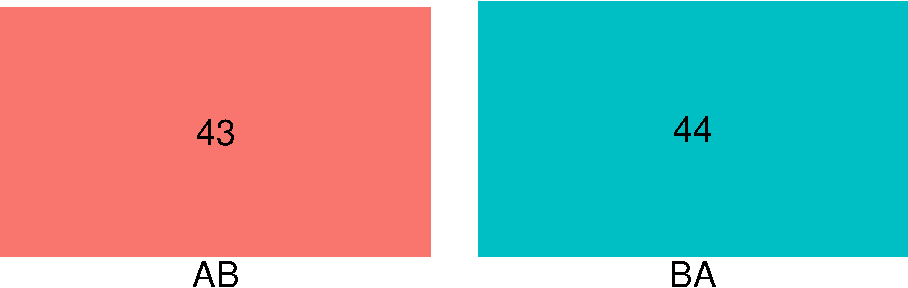
\includegraphics{40-EDA1_files/figure-pdf/fig-groups-1.pdf}

}

\caption{\label{fig-groups}Estudiantes asignados a cada grupo.}

\end{figure}

El campo \texttt{LastTry} contiene la fecha y hora de realización del
test. Con esta información podemos conocer el tiempo que empleó cada
estudiante entre subtitulados. La Tabla~\ref{tbl-washout} muestra que
hay algunos test que se hicieron demasiado rápido \footnote{Hay que
  tener en cuenta que la duración de vídeo es de algo más de 40 segundos
  y que los estudiantes tienen que contestar un test de 18 preguntas.}.

\hypertarget{tbl-washout}{}
\begin{longtable}{c}
\caption{\label{tbl-washout}Tiempos de realización de la segunda actividad de duración inferior a 2
minutos. }\tabularnewline

\toprule
Minutes \\ 
\midrule
0.93 \\ 
1.3 \\ 
1.7 \\ 
1.72 \\ 
1.78 \\ 
1.97 \\ 
\bottomrule
\end{longtable}

La Figura~\ref{fig-distinct} muestra que hay 28 test en los que el
estudiante contestó a todas las preguntas usando únicamente 2 respuestas
diferentes. Además hay 13 test en los que se contestaron todas las
preguntas con 1 respuesta.

\begin{figure}[h]

{\centering 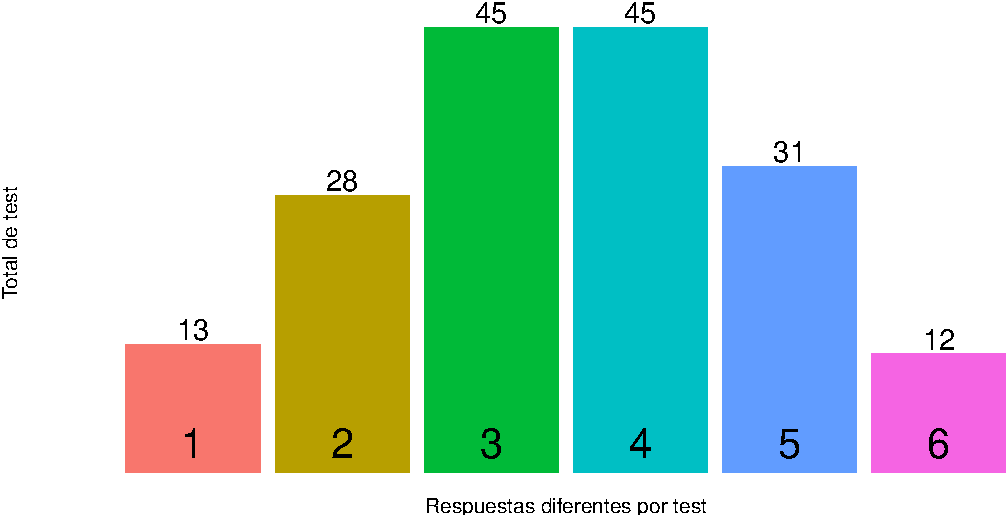
\includegraphics{40-EDA1_files/figure-pdf/fig-distinct-1.pdf}

}

\caption{\label{fig-distinct}Número de respuestas diferentes en un mismo
test.}

\end{figure}

\clearpage

La tabla Tabla~\ref{tbl-distinct2} muestra la respuesta utilizada, el
grupo y el periodo de los test con respuesta única.

\hypertarget{tbl-distinct2}{}
\begin{longtable}{rlr}
\caption{\label{tbl-distinct2}Test en los que todas las preguntas se contestan el mismo valor de
respuesta. }\tabularnewline

\toprule
Response & Seq & Test \\ 
\midrule
2 & AB & 01 \\ 
2 & AB & 02 \\ 
3 & BA & 01 \\ 
3 & BA & 02 \\ 
3 & BA & 02 \\ 
3 & BA & 02 \\ 
4 & AB & 01 \\ 
4 & AB & 01 \\ 
4 & AB & 02 \\ 
4 & BA & 01 \\ 
4 & BA & 02 \\ 
4 & BA & 02 \\ 
4 & BA & 02 \\ 
\bottomrule
\end{longtable}

La Figura~\ref{fig-compare} presenta la distribución de la cantidad de
respuestas cuyo valor cambia entre los dos test que realiza cada
estudiante.

\begin{figure}[h]

{\centering 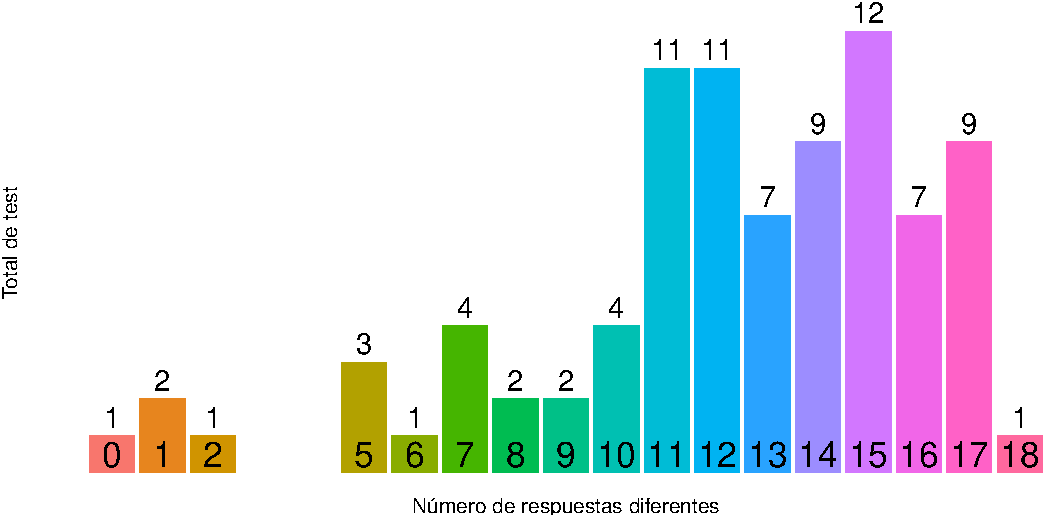
\includegraphics{40-EDA1_files/figure-pdf/fig-compare-1.pdf}

}

\caption{\label{fig-compare}Número de respuestas diferentes entre los
test para cada estudiante.}

\end{figure}

\clearpage

Tan solo 1 estudiante respondió a todas las preguntas con el mismo valor
en los dos test. Por otro lado, no hay test que tengan un número
excesivo de contestaciones \enquote{No sé/No contesto} (ver
Tabla~\ref{tbl-noanswer}).

\hypertarget{tbl-noanswer}{}
\begin{longtable}{rr}
\caption{\label{tbl-noanswer}Los 5 test con más respuestas `No sé/No contesto' }\tabularnewline

\toprule
Test & Total respuesta por test \\ 
\midrule
01 & 5 \\ 
01 & 5 \\ 
02 & 5 \\ 
02 & 5 \\ 
01 & 4 \\ 
\bottomrule
\end{longtable}

\hypertarget{conclusiones.}{%
\subsubsection{Conclusiones.}\label{conclusiones.}}

No parece razonable realizar la actividad en menos de 2 minutos. Se
observa que en algunos test hay poca variabilidad. Sin embargo, no son
muchos los test con estas características así que se ha decidido
mantener estos datos a pesar de que se pueda dubar de si en ellos los
estudiantes contestaron con la debida atención y diligencia.

\hypertarget{valores-nulos-o-erruxf3neos.}{%
\subsection{Valores nulos o
erróneos.}\label{valores-nulos-o-erruxf3neos.}}

En los test no se ha detectado ningún valor nulo ni erróneo. Sin embargo
tenemos algunos de estos valores en la información socioeconómica de los
estudiantes (ver Tabla~\ref{tbl-contingencia}).

\begin{table}

\caption{\label{tbl-contingencia}Tablas de contingencia de la
información socioeconómica de los
estudiantes.}\begin{minipage}[t]{0.50\linewidth}

{\centering 

\hypertarget{tbl-contingencia-1}{}
\begin{longtable}{cr}
\tabularnewline

\toprule
gender & Freq \\ 
\midrule
f & 92 \\ 
m & 38 \\ 
NA & 44 \\ 
\bottomrule
\end{longtable}

Estudiantes por sexo.

}

\end{minipage}%
%
\begin{minipage}[t]{0.50\linewidth}

{\centering 

\hypertarget{tbl-contingencia-2}{}
\begin{longtable}{cr}
\tabularnewline

\toprule
year\_of\_birth & Freq \\ 
\midrule
None & 44 \\ 
NA & 2 \\ 
\bottomrule
\end{longtable}

Estudiantes con valor nulo en el campo año de nacimiento.

}

\end{minipage}%
\newline
\begin{minipage}[t]{0.50\linewidth}

{\centering 

\hypertarget{tbl-contingencia-3}{}
\begin{longtable}{cr}
\tabularnewline

\toprule
level\_of\_education & Freq \\ 
\midrule
a & 50 \\ 
b & 16 \\ 
hs & 4 \\ 
m & 30 \\ 
other & 4 \\ 
p & 20 \\ 
NA & 50 \\ 
\bottomrule
\end{longtable}

Estudiantes por nivel educativo.

}

\end{minipage}%
%
\begin{minipage}[t]{0.50\linewidth}

{\centering 

\hypertarget{tbl-contingencia-4}{}
\begin{longtable}{cr}
\tabularnewline

\toprule
level\_of\_knowledge & Freq \\ 
\midrule
4 & 2 \\ 
6 & 4 \\ 
7 & 30 \\ 
8 & 44 \\ 
9 & 40 \\ 
10 & 32 \\ 
NA & 22 \\ 
\bottomrule
\end{longtable}

Estudiantes en función del número de preguntas acertadas en el test de
conocimiento.

}

\end{minipage}%

\end{table}

\hypertarget{sec-eda-3}{%
\section{\texorpdfstring{Comparación de los tratamientos \(A\) y \(B\)
entre
grupos.}{Comparación de los tratamientos A y B entre grupos.}}\label{sec-eda-3}}

La Figura~\ref{fig-diff} presenta una forma de comparar los dos test que
realizados por los estudiantes. Para cada estudiante se comparó pregunta
a pregunta sus dos test y se contabilizó la diferencia entre el número
de preguntas en que la puntuación en el segundo vídeo fue superior y en
las que lo fue inferior (las que no variaron de puntuación no se
consideraron). En el eje \(x\) se muestra la diferencia entre preguntas.
Cantidades negativas indican que hay más respuestas en el segundo de los
test que han empeorado respecto al primero de las que han mejorado. En
el eje \(y\) se representa el número de estudiantes para cada
diferencia. Esta frecuencia se representa en negativo cuando la
diferencia es negativa \footnote{En la comparación se han omitido
  aquellas preguntas en las que el estudiante contestó \enquote{No sé/No
  contesto} en la pregunta correspondiente de uno de los test.}. Esto es
una forma de evaluar si el estudiante valoró mejor o no el segundo vídeo
que el primero.

\begin{figure}[h]

{\centering 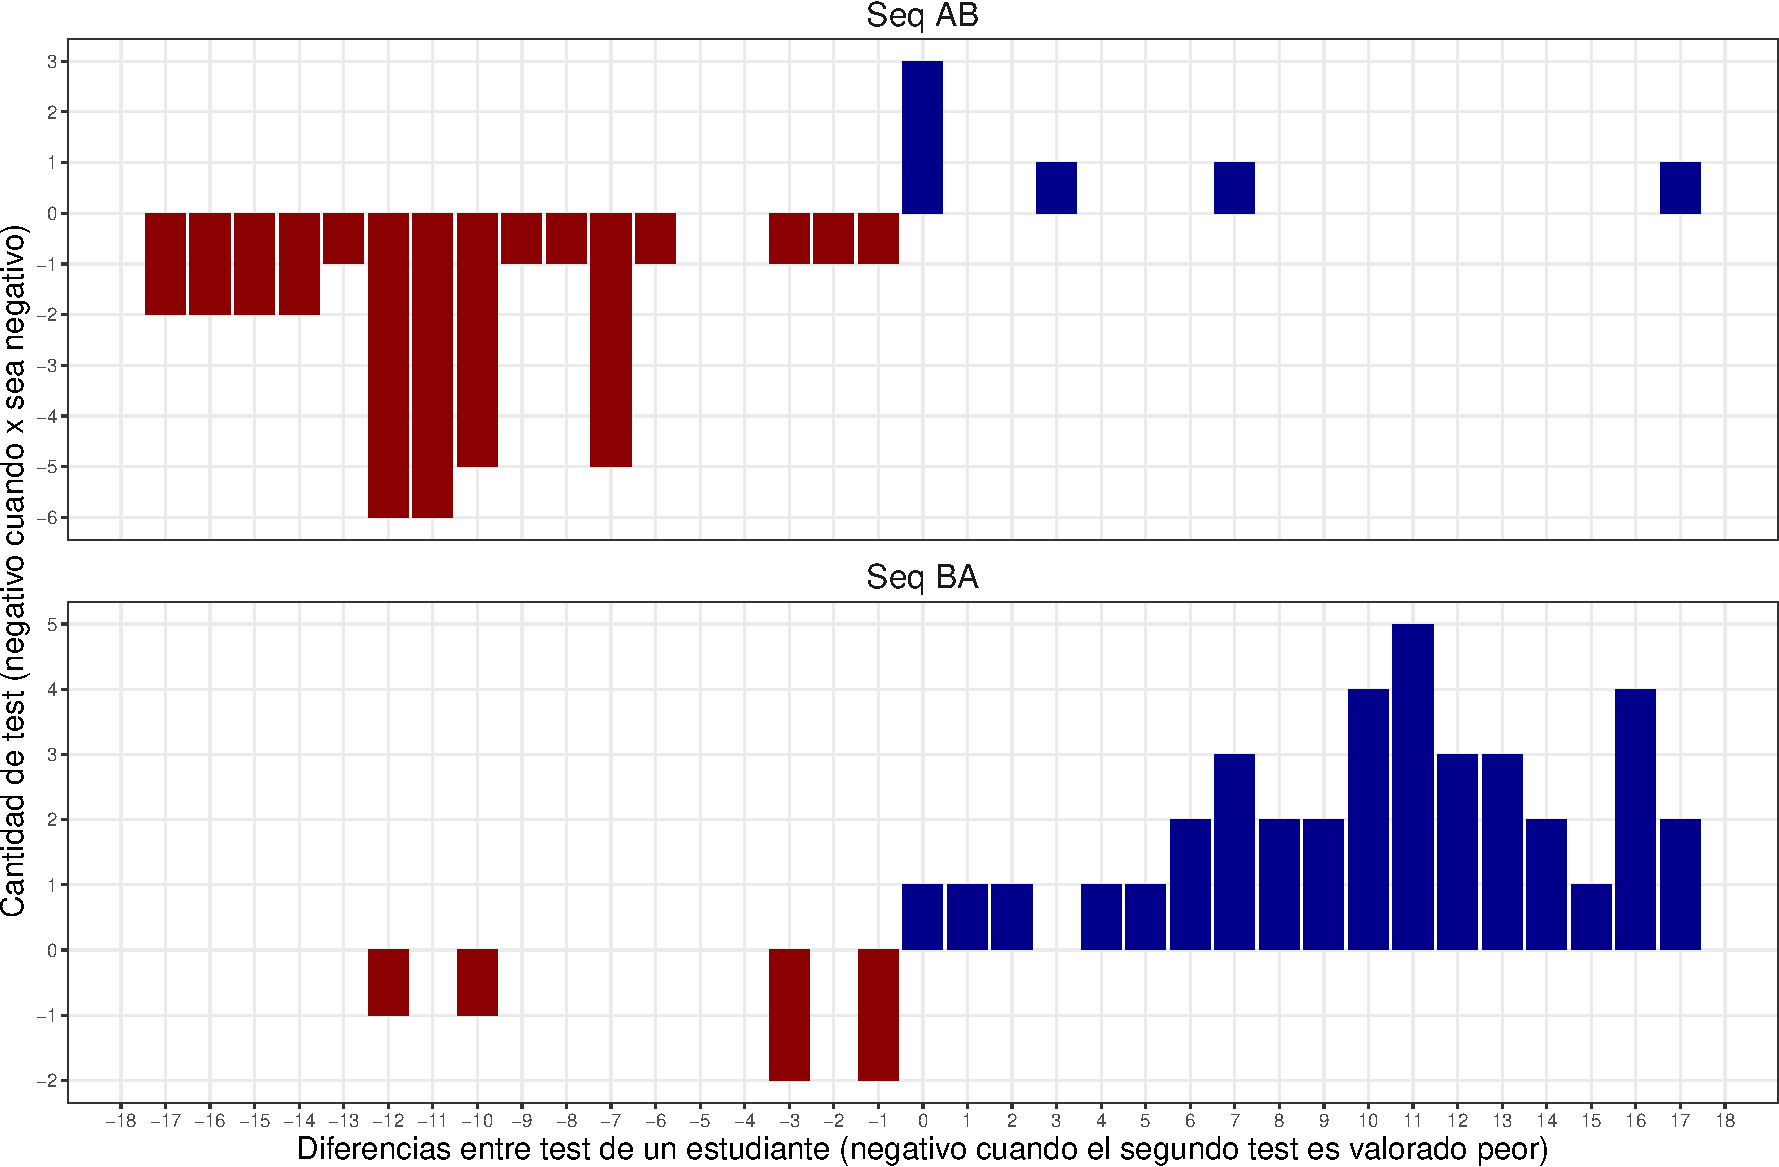
\includegraphics{40-EDA1_files/figure-pdf/fig-diff-1.pdf}

}

\caption{\label{fig-diff}Frecuencias absolutas de las diferencias en las
respuestas entre test por estudiante y grupo.}

\end{figure}

Vemos que en el grupo \(AB\) las diferencias tienden a ser negativas y
en el \(BA\) positivas. Esto estaría indicando que los estudiantes
valoran mejor el subtitulado de nivel \(A\). Por ello es esperable que
las respuestas de los estudiantes del grupo \(AB\) hayan empeorado y que
las diferencias sean negativas y que lo contrario haya sucedido con las
del grupo \(BA\). La diferencia más frecuente en el grupo \(AB\) es 12 y
en el grupo \(BA\) este valor es 11.

Resulta llamativo que haya estudiantes cuyas contestaciones estén tan
alejadas de la tendencia de su grupo. En la Tabla~\ref{tbl-diff} se
muestran los tiempos que han transcurrido entre la realización de los
test de aquellos estudiantes cuyas respuestas difieren de forma
importante de su grupo. Se observa que casi todos son tiempos entre
actividades muy cortos. En cualquier caso y, como no son muchos, se ha
decidido no eliminarlos y realizar el análisis con ellos.

\hypertarget{tbl-diff}{}
\begin{longtable}{lrc}
\caption{\label{tbl-diff}Estudiantes que tienen diferencias en sus respuestas muy alejadas de la
tendencia de su grupo. }\tabularnewline

\toprule
Seq & Diff & Minutes \\ 
\midrule
AB & 17 & 1.3 \\ 
AB & 7 & 3.33 \\ 
BA & -10 & 50345.95 \\ 
BA & -12 & 1.7 \\ 
\bottomrule
\end{longtable}

En la Figura~\ref{fig-freqs} representamos la frecuencia relativa del
valor de respuesta para cada grupo y test en todas la preguntas. Esta es
otra forma de comparar los niveles de subtitulado.

La Figura~\ref{fig-freqs} muestra algunas cuestiones interesantes:

\begin{itemize}
\item
  El tratamiento (subtitulado) con nivel \(A\) presenta claramente
  mayores valores de respuesta que el \(B\) como ya habíamos visto (ver
  Figura~\ref{fig-diff}). Si en este momento tuviéramos que decidir qué
  subtitulado es cada uno parece claro que sería el de nivel \(A\). No
  obstante, ni en el análisis exploratorio ni en el modelado estadístico
  se hará ninguna suposición.
\item
  En general los dos grupos muestran bastante acuerdo en el subtitulado
  en ambos niveles: En el nivel de tratamiento \(A\) los dos grupos
  tienen una frecuencia relativa similar de respuestas positivas
  (valores 4 y 5). El grupo \(AB\) tiene un 82\% de respuestas positivas
  frente a un 84\% el grupo \(BA\). No obstante, el grupo \(AB\) tiene
  más respuestas con valor 5 que el grupo \(BA\) (56\% frente a 41\%).
  La valoración es también similar entre grupos en el nivel de
  tratamiento \(B\): el grupo \(AB\) tiene 44\% de respuestas positivas
  y 47\% el grupo \(BA\). Las valoraciones negativas (1, 2), la neutra
  (3) y la \enquote*{No sé / No contesto} (0) son también muy similares.
\item
  Las respuestas son similares entre periodos aunque ligeramente más
  negativas en el segundo. Así un 65\% de las respuestas son positivas
  en el primer periodo frente a un 64\% en el segundo.
\end{itemize}

\begin{figure}[h]

{\centering 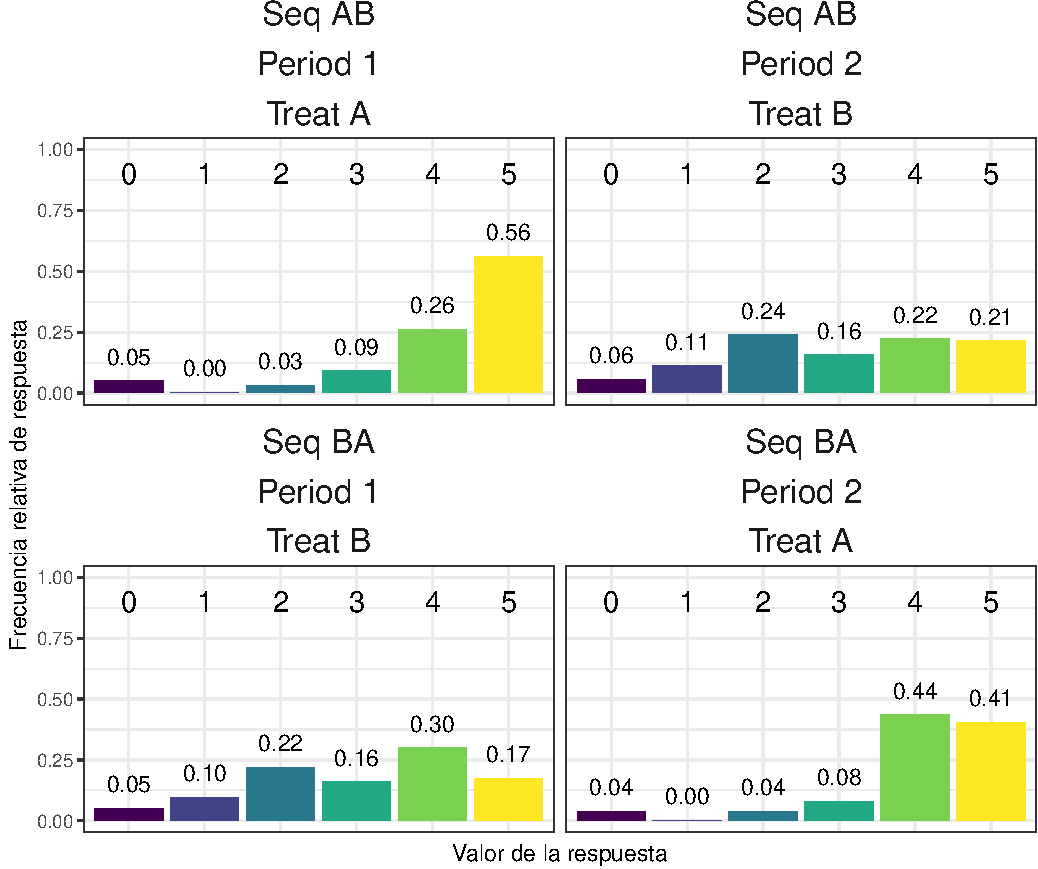
\includegraphics{40-EDA1_files/figure-pdf/fig-freqs-1.pdf}

}

\caption{\label{fig-freqs}Frecuencias relativas de las respuestas al
test.}

\end{figure}

El análisis marginalizado de tratamiento, secuencia y periodo tiene
estos resultados referidos a las preguntas con contestación positiva (4,
5):

\begin{itemize}
\item
  El tratamiento \(A\) tiene un 83\% marginalizado de respuestas
  positivas frente al 46\% del tratamiento \(B\).
\item
  El periodo 1 tiene un 65\% marginalizado de respuestas positivas
  frente al 64\% del periodo 2.
\item
  Finalmente, la secuencia \(AB\) tiene un 63\% de respuestas positivas
  frente 66\% de la secuencia \(BA\). Analizado por respuestas
  individuales, la respuesta 4 pasa de 24\% en la secuencia \(AB\) a
  37\% en la \(BA\) y, de forma contraria, en la respuesta 5 pasa de
  39\% en \(AB\) a 29\% en \(BA\). En las respuestas negativas y no
  contestadas y neutra no se aprecian estas variaciones.
\end{itemize}

\hypertarget{anuxe1lisis-de-las-preguntas.}{%
\section{Análisis de las
preguntas.}\label{anuxe1lisis-de-las-preguntas.}}

El gráfico Figura~\ref{fig-levels} muestra la frecuencia relativa por
grupo y por test de las preguntas clasificadas por niveles de respuesta,
considerando que:

\begin{itemize}
\tightlist
\item
  Los niveles 1 y 2 se consideran valoraciones negativas.
\item
  El nivel 3 se considera neutro.
\item
  Los niveles 4 y 5 se consideran positivos.
\item
  El nivel 0 (\enquote{No sé / No contesto}) se excluye en este
  análisis.
\end{itemize}

Se muestra en primer lugar la pregunta 18 por ser una valoración global
del subtitulado y que resume la opinión que sobre el mismo tiene el
estudiante. Volvemos a constatar que el subtitulado \(A\) es mejor
valorado por los estudiantes, pero ahora vemos que en las 18 preguntas
ambos grupos tienen mas puntuaciones positivas y menos negativas en el
subtitulado \(A\) que el \(B\). También volvemos a encontrar que los dos
grupos valoran de forma muy similar los dos niveles de subtitulado en
todas la preguntas. En el nivel de subtitulado \(A\) las preguntas
\(Q15\), \(Q16\) y \(Q17\) obtienen relativamente peores valoraciones
(consultar la Tabla~\ref{tbl-likert-scale} para ver los valores) y estas
son similares en ambos subtitulados. Hay algunas preguntas que son
valoradas de forma positiva incluso en el nivel de subtitulado \(B\)
(por ejemplo \(Q04\) o \(Q13\)) y que, por lo tanto, su valoración es
similar en ambos subtitulados. Por último, las preguntas \(Q05\) y
\(Q09\) (también la \(Q14\) pero solo para el grupo \(BA\)) tienen una
valoración muy negativa en el nivel de subtitulado \(B\).

\begin{figure}[h]

{\centering 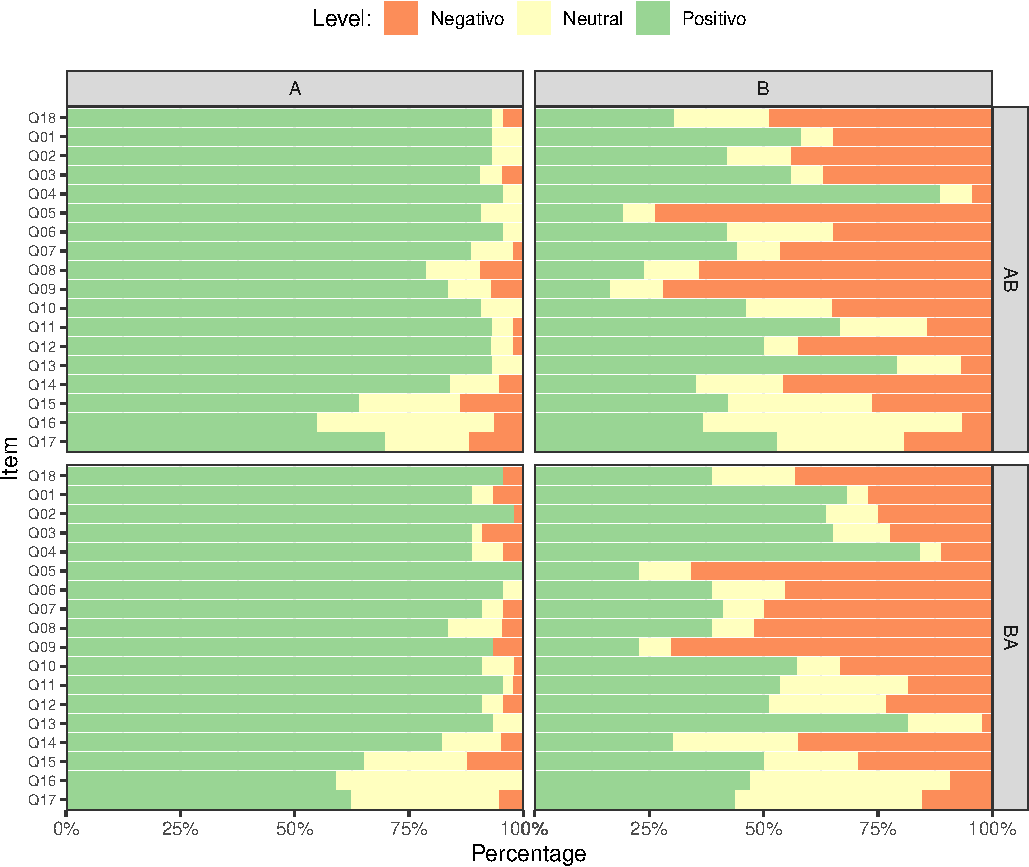
\includegraphics{40-EDA1_files/figure-pdf/fig-levels-1.pdf}

}

\caption{\label{fig-levels}Frecuencias relativas de las respuestas por
pregunta.}

\end{figure}

La figura Figura~\ref{fig-likert} clasifica la preguntas por valoración
y permite constatar lo que ya habíamos visto en el párrafo anterior con
mayor comodidad.

\begin{figure}

\begin{minipage}[t]{0.50\linewidth}

{\centering 

\raisebox{-\height}{

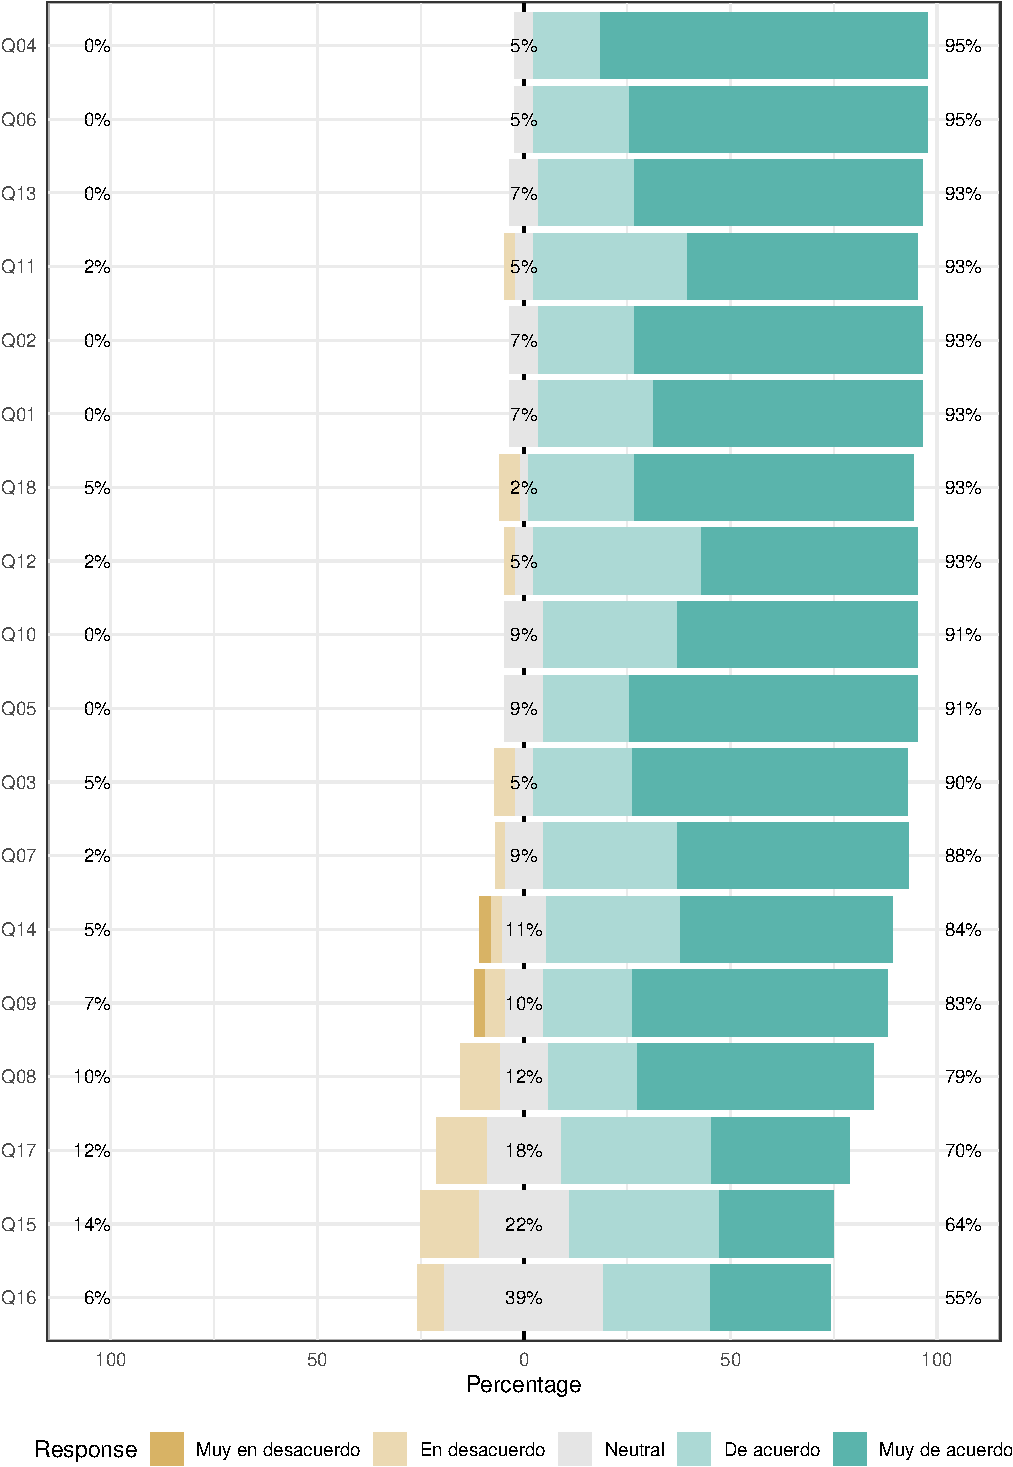
\includegraphics{40-EDA1_files/figure-pdf/fig-likert-1.pdf}

}

}

\subcaption{\label{fig-likert-1}Seq AB , Treat A}
\end{minipage}%
%
\begin{minipage}[t]{0.50\linewidth}

{\centering 

\raisebox{-\height}{

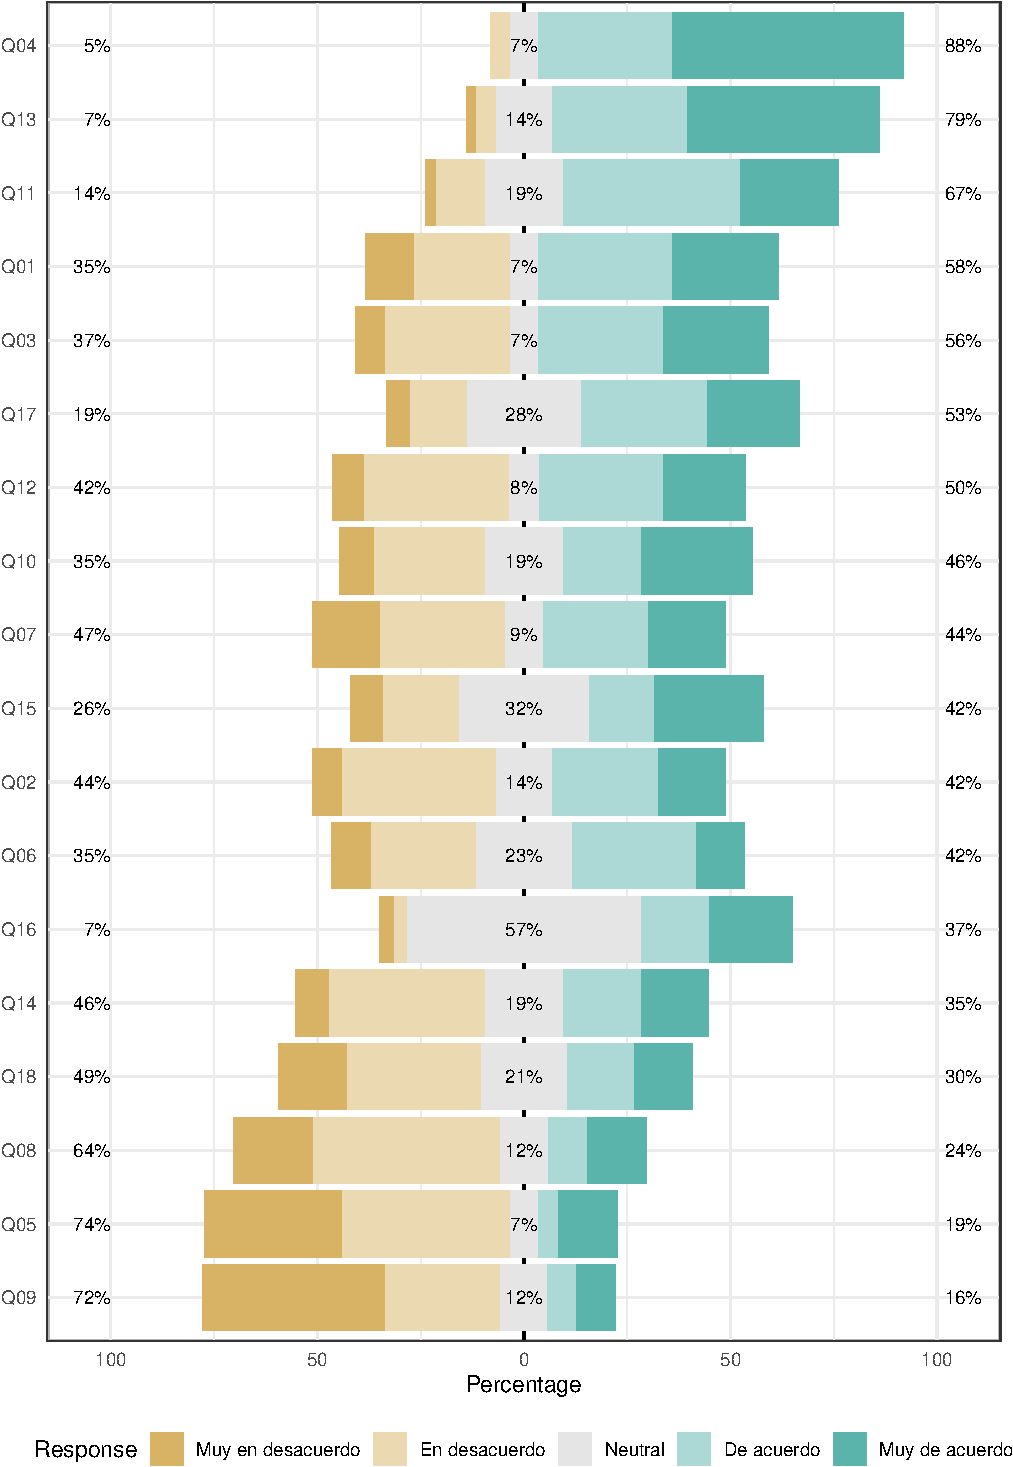
\includegraphics{40-EDA1_files/figure-pdf/fig-likert-2.pdf}

}

}

\subcaption{\label{fig-likert-2}Seq AB , Treat B}
\end{minipage}%
\newline
\begin{minipage}[t]{0.50\linewidth}

{\centering 

\raisebox{-\height}{

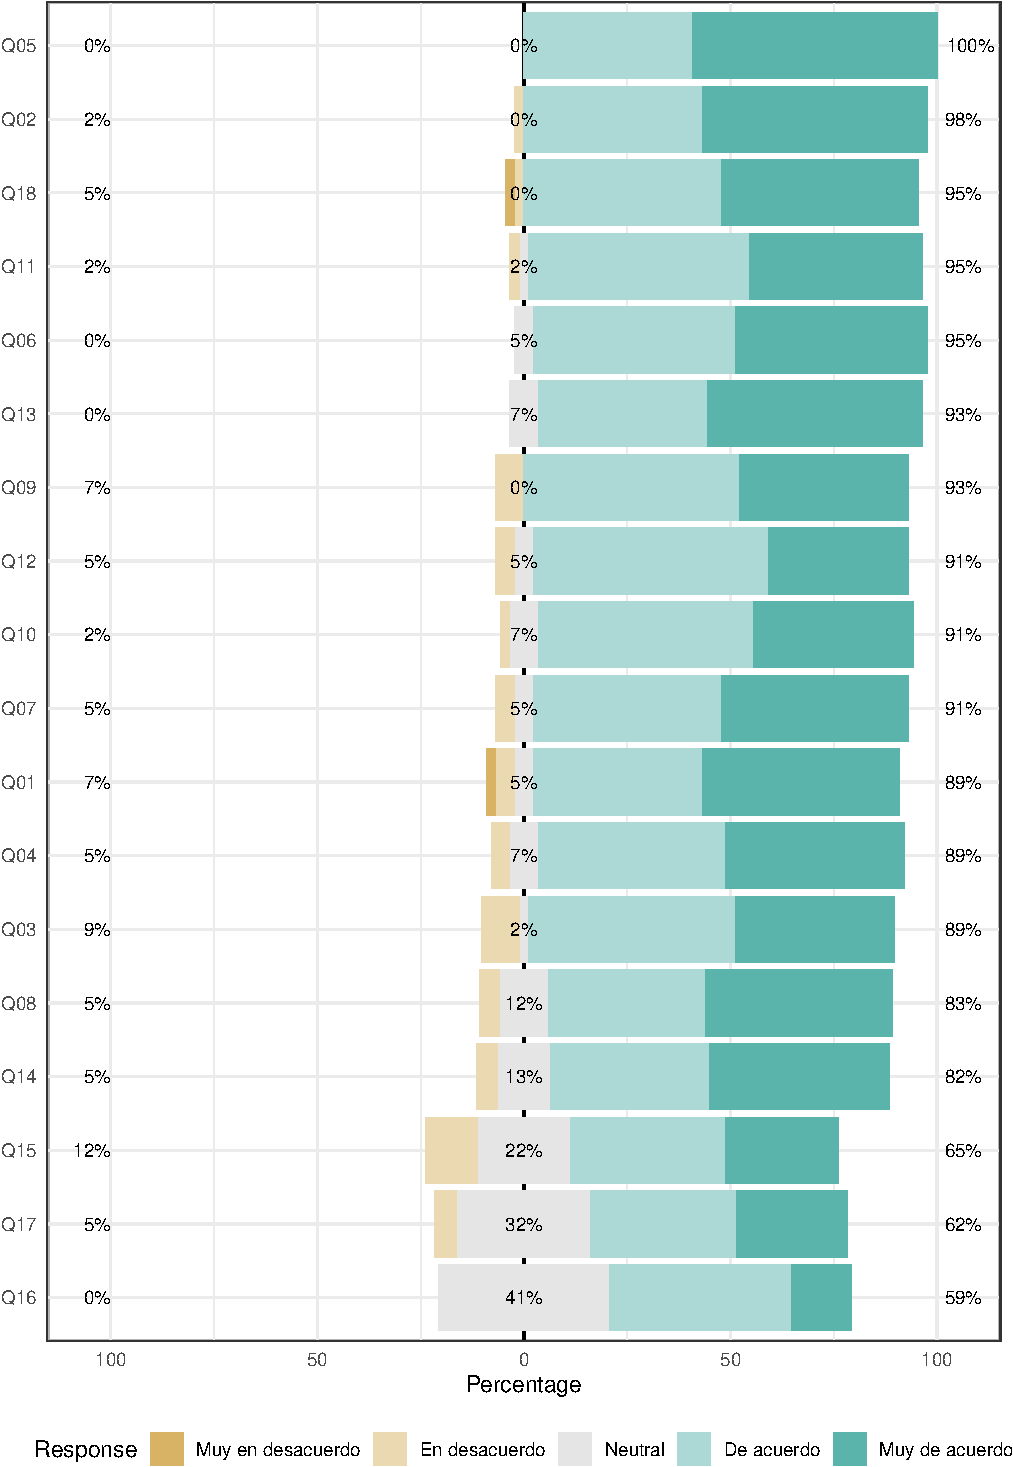
\includegraphics{40-EDA1_files/figure-pdf/fig-likert-3.pdf}

}

}

\subcaption{\label{fig-likert-3}Seq BA , Treat A}
\end{minipage}%
%
\begin{minipage}[t]{0.50\linewidth}

{\centering 

\raisebox{-\height}{

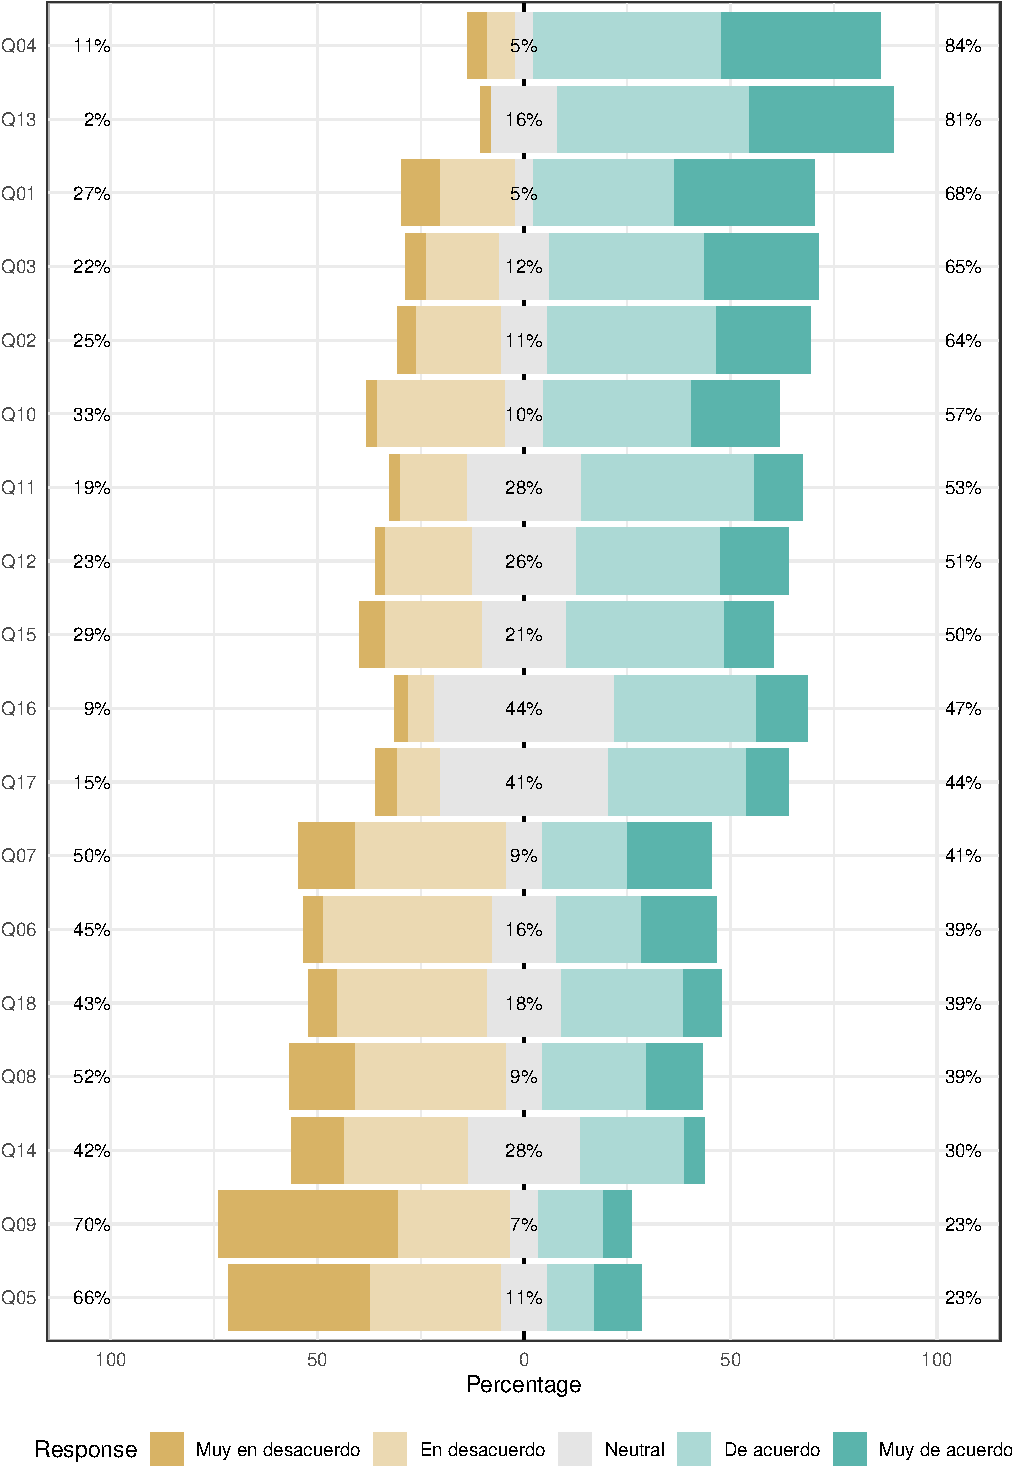
\includegraphics{40-EDA1_files/figure-pdf/fig-likert-4.pdf}

}

}

\subcaption{\label{fig-likert-4}Seq BA , Treat B}
\end{minipage}%

\caption{\label{fig-likert}Preguntas ordenadas por valoración.}

\end{figure}

\bookmarksetup{startatroot}

\hypertarget{sec-analisis}{%
\chapter{Análisis estadístico.}\label{sec-analisis}}

\hypertarget{sec-cluster}{%
\section{Agrupamientos de preguntas.}\label{sec-cluster}}

\hypertarget{sec-cronbach}{%
\subsection{Correlación entre preguntas con el alfa de
Cronbach.}\label{sec-cronbach}}

Normalmente las preguntas de un cuestionario pretenden medir una
variable que está oculta o latente. En nuestro caso es la calidad del
subtitulado. Las respuestas a estas preguntas relacionadas deben ser
consistentes internamente, es decir, las respuestas deben
correlacionarse fuerte y positivamente.

Un índice que se utiliza habitualmente para medir la consistencia
interna de un cuestionario es el coeficiente
\texttt{alfa\ de\ Cronbach}, ver \textcite{schweinberger2020survey}. Se
define de esta forma:

\begin{equation}
\alpha = \frac{N}{N-1} \left(1 - \frac{\sum_{i=1}^{N} s_{i}^{2}}{s^{2}} \right)
\end{equation}

Donde:

\begin{itemize}
\tightlist
\item
  \(\alpha\) es el coeficiente \texttt{alfa\ de\ Cronbach}.
\item
  \(N\) es el número de items de la escala de Likert.
\item
  \(s_{i}^{2}\) es la varianza de la puntuación del item \(i\).
\item
  \(s^{2}\) es la varianza total de las puntuaciones de todos los items.
\end{itemize}

Valores cercanos 1 indican una fuerte correlación en las respuestas y se
admite que las preguntas del cuestionario están midiendo la misma
variable latente.

Para calcular en R este coeficiente podemos usar la función
\texttt{alpha} del paquete \texttt{psych}:

\scriptsize

\begin{Shaded}
\begin{Highlighting}[]
\NormalTok{alpha }\OtherTok{\textless{}{-}}\NormalTok{ df\_all }\SpecialCharTok{\%\textgreater{}\%}
    \FunctionTok{pivot\_wider}\NormalTok{(}
        \AttributeTok{names\_from =}\NormalTok{ Question,}
        \AttributeTok{values\_from =}\NormalTok{ Response\_v,}
        \AttributeTok{id\_cols =} \FunctionTok{c}\NormalTok{(Treat, Subject)}
\NormalTok{    ) }\SpecialCharTok{\%\textgreater{}\%}
\NormalTok{    dplyr}\SpecialCharTok{::}\FunctionTok{select}\NormalTok{(}\SpecialCharTok{{-}}\FunctionTok{c}\NormalTok{(Treat, Subject)) }\SpecialCharTok{\%\textgreater{}\%}
\NormalTok{    psych}\SpecialCharTok{::}\FunctionTok{alpha}\NormalTok{()}
\end{Highlighting}
\end{Shaded}

\normalsize

Se obtiene un coeficiente alfa de \texttt{alfa\ de\ Cronbach} de 0.92
que indica una muy buena correlación entre las respuestas a todas las
preguntas. Este valor apenas se ve alterado si se elimina una de las
preguntas (ver Tabla~\ref{tbl-drop-alpha}).

\scriptsize

\begin{table}

\caption{\label{tbl-drop-alpha}Valor del coeficiente alpha de Cronbach
si se elimina una pregunta.}\begin{minipage}[t]{\linewidth}
\subcaption{\label{tbl-drop-alpha-1}}

{\centering 

\begin{longtable*}{rrrrrrrrr}
\toprule
Q18 & Q01 & Q02 & Q03 & Q04 & Q05 & Q06 & Q07 & Q08 \\ 
\midrule
0.91 & 0.92 & 0.92 & 0.92 & 0.92 & 0.91 & 0.91 & 0.91 & 0.91 \\ 
\bottomrule
\end{longtable*}

}

\end{minipage}%
\newline
\begin{minipage}[t]{\linewidth}
\subcaption{\label{tbl-drop-alpha-2}}

{\centering 

\begin{longtable*}{rrrrrrrrr}
\toprule
Q09 & Q10 & Q11 & Q12 & Q13 & Q14 & Q15 & Q16 & Q17 \\ 
\midrule
0.91 & 0.91 & 0.92 & 0.91 & 0.92 & 0.92 & 0.92 & 0.93 & 0.92 \\ 
\bottomrule
\end{longtable*}

}

\end{minipage}%

\end{table}

\normalsize

En la Tabla~\ref{tbl-item-alpha} mostramos las preguntas que más
contribuyen al índice \texttt{alpha\ de\ Cronbach}. Es interesante que
la pregunta \(Q18\), que es la valoración general del cuestionario, sea
la que mejor contribución tiene al índice.

\scriptsize

\begin{table}

\caption{\label{tbl-item-alpha}Relación de cada pregunta con el índice
alpha de Cronbach.}\begin{minipage}[t]{\linewidth}
\subcaption{\label{tbl-item-alpha-1}}

{\centering 

\begin{longtable*}{rrrrrrrrr}
\toprule
Q18 & Q05 & Q06 & Q09 & Q08 & Q07 & Q10 & Q12 & Q02 \\ 
\midrule
0.86 & 0.81 & 0.79 & 0.79 & 0.77 & 0.75 & 0.73 & 0.72 & 0.71 \\ 
\bottomrule
\end{longtable*}

}

\end{minipage}%
\newline
\begin{minipage}[t]{\linewidth}
\subcaption{\label{tbl-item-alpha-2}}

{\centering 

\begin{longtable*}{rrrrrrrrr}
\toprule
Q03 & Q14 & Q01 & Q11 & Q15 & Q13 & Q04 & Q16 & Q17 \\ 
\midrule
0.68 & 0.66 & 0.65 & 0.64 & 0.56 & 0.51 & 0.46 & 0.44 & 0.42 \\ 
\bottomrule
\end{longtable*}

}

\end{minipage}%

\end{table}

\normalsize

\clearpage

\hypertarget{sec-cluster2}{%
\subsection{Agrupamiento jerárquico aglomerativo.}\label{sec-cluster2}}

En en la Sección~\ref{sec-cronbach} y en la Sección~\ref{sec-eda-3}
hemos visto que algunas de las preguntas tienen respuestas similares a
otras pero diferentes del resto. Puede ser interesante aplicar una
técnica de agrupamiento que nos permita crear grupos de preguntas que
podremos analizar por separado.

Vamos a realizar una agrupación jerárquica aglomerativa de las preguntas
en función de la tabla de contingencia de las respuestas utilizando la
distancia euclidea como medida de distancia y el método de aglomeración
de enlace completo para unir conglomerados \footnote{El método de enlace
  completo usa la distancia máxima entre dos conglomerados para
  seleccionar los más cercanos a unir.}. Para ello primero calculamos la
tabla de contingencia (ver Tabla~\ref{tbl-contingencia}) de preguntas y
respuestas.

\begin{Shaded}
\begin{Highlighting}[]
\NormalTok{table }\OtherTok{\textless{}{-}}\NormalTok{ df\_all }\SpecialCharTok{\%\textgreater{}\%}
    \FunctionTok{xtabs}\NormalTok{(}\SpecialCharTok{\textasciitilde{}}\NormalTok{ Question }\SpecialCharTok{+}\NormalTok{ Response, }\AttributeTok{data =}\NormalTok{ .)}
\end{Highlighting}
\end{Shaded}

\scriptsize

\hypertarget{tbl-contingencia}{}
\begin{longtable}{crrrrrr}
\caption{\label{tbl-contingencia}Tabla de contingencia de preguntas y respuestas. }\tabularnewline

\toprule
Question & Response\_0 & Response\_1 & Response\_2 & Response\_3 & Response\_4 & Response\_5 \\ 
\midrule
Q18 & 0 & 11 & 33 & 18 & 52 & 60 \\ 
Q01 & 0 & 10 & 20 & 10 & 59 & 75 \\ 
Q02 & 0 & 5 & 26 & 14 & 58 & 71 \\ 
Q03 & 5 & 5 & 26 & 11 & 60 & 67 \\ 
Q04 & 0 & 2 & 7 & 10 & 61 & 94 \\ 
Q05 & 1 & 29 & 31 & 12 & 34 & 67 \\ 
Q06 & 1 & 6 & 29 & 21 & 53 & 64 \\ 
Q07 & 0 & 13 & 32 & 14 & 54 & 61 \\ 
Q08 & 4 & 15 & 41 & 19 & 40 & 55 \\ 
Q09 & 1 & 39 & 29 & 12 & 42 & 51 \\ 
Q10 & 8 & 4 & 24 & 18 & 59 & 61 \\ 
Q11 & 3 & 2 & 14 & 23 & 75 & 57 \\ 
Q12 & 5 & 4 & 26 & 18 & 69 & 52 \\ 
Q13 & 1 & 2 & 2 & 19 & 62 & 88 \\ 
Q14 & 21 & 9 & 29 & 27 & 44 & 44 \\ 
Q15 & 26 & 5 & 25 & 36 & 47 & 35 \\ 
Q16 & 47 & 2 & 5 & 57 & 39 & 24 \\ 
Q17 & 29 & 4 & 15 & 44 & 49 & 33 \\ 
\bottomrule
\end{longtable}

\normalsize

Con la tabla de contingencia calculamos las distancias entre preguntas y
realizamos el agrupamiento. En el dendograma se aprecian claramente tres
agrupamientos. Es muy interesante constatar que los tres grupos están
formados por preguntas que en su mayor parte son correlativas. Esto es
consistente con que al elaborar un test normalmente se colocan las
preguntas por unidades temáticas y con que el encuestado también suele
hacerlo teniendo en cuenta esta estructura y tiende a responder de forma
similar a las preguntas correlativas.

\begin{Shaded}
\begin{Highlighting}[]
\NormalTok{dist }\OtherTok{\textless{}{-}} \FunctionTok{dist}\NormalTok{(table, }\AttributeTok{method =} \StringTok{"euclidean"}\NormalTok{)}
\NormalTok{cluster }\OtherTok{\textless{}{-}} \FunctionTok{hclust}\NormalTok{(dist, }\AttributeTok{method =} \StringTok{"complete"}\NormalTok{)}
\FunctionTok{plot}\NormalTok{(cluster)}
\end{Highlighting}
\end{Shaded}

\begin{figure}[h]

{\centering 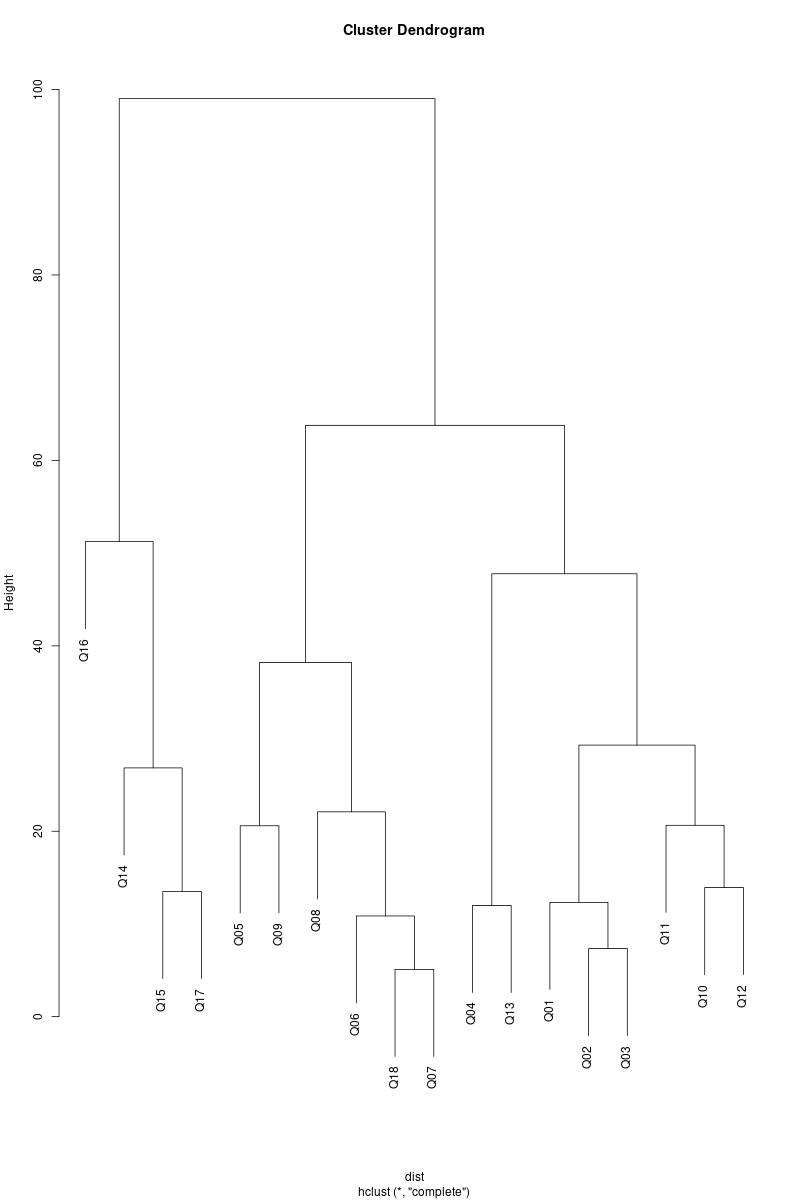
\includegraphics[width=4.16667in,height=\textheight]{images/cluster.png}

}

\caption{Dendograma de aglomeramiento jerárquico de preguntas en función
de la tabla de contingencia de respuestas.}

\end{figure}

Podemos distinguir los siguientes grupos y subgrupos:

\begin{itemize}
\tightlist
\item
  Grupo 1: Trata sobre la corrección del subtítulo.

  \begin{itemize}
  \tightlist
  \item
    Subgrupo 05, 06, 07, 08, 09: Preguntas sobre si la información que
    presenta el subtítulo es correcta y está bien escrita.
  \item
    Pregunta 18: Valoración general del subtitulado. El que esta
    pregunta esté incluida en el grupo sobre corrección estaría
    indicando que este es el apartado al que más importancia dan los
    estudiantes a la hora de valorar la calidad del subtitulado.
  \end{itemize}
\item
  Grupo 2: Es el más numeroso. En general está formado por preguntas
  sobre el grado de dificultad que presenta la lectura del subtítulo.

  \begin{itemize}
  \tightlist
  \item
    Subgrupo preguntas Q01, Q02, Q03: Colocación de los subtítulos.
  \item
    Subgrupo preguntas Q10, Q11, Q12: Sincronización, velocidad y número
    de líneas.
  \item
    Subgrupo preguntas Q04, Q13: Contraste y legibilidad.
  \end{itemize}
\item
  Grupo 3: Son preguntas que tratan también sobre la corrección del
  subtítulo, pero con la diferencia sobre el grupo uno de que se trata
  de cuestiones más sutiles y presumiblemente más difíciles de valorar
  por un novato. Está formado por las preguntas Q14, Q15, Q16 y Q17.
\end{itemize}

\hypertarget{anuxe1lisis-de-tablas-de-contingencia.}{%
\section{Análisis de tablas de
contingencia.}\label{anuxe1lisis-de-tablas-de-contingencia.}}

En esta sección se aplicarán técnicas estadísticas que se basan en
tablas de contingencia. Una descripción teórica de este tipo de técnicas
se pueden encontrar en \textcite{agresti_2018}. Un tratamiento aplicado
y basado en gráficos, que será el enfoque que seguiremos en este
trabajo, es realizado en \textcite{frienly2015}.

\hypertarget{comparaciuxf3n-mediante-mosaicos.}{%
\subsection{Comparación mediante
mosaicos.}\label{comparaciuxf3n-mediante-mosaicos.}}

En el Figura~\ref{fig-mosaic} se representan en forma de mosaico las
tablas de contingencia de las respuestas por tratamiento y secuencia. La
información mostrada es similar a la que presentamos en la
Figura~\ref{fig-freqs}, aunque el gráfico es más intuitivo ya que la
anchura y altura de los rectángulos son proporcionales a la frecuencia
marginal de la secuencia y el tratamiento respectivamente y el área es
proporcional a la frecuencia conjunta. En esta ocasión hemos decidido
emparejar los tratamientos en lugar de hacerlo con la secuencia, como
hicimos anteriormente. Esto permite una mejor comparación de las
diferencias entre grupos. Con ello podemos ver fácilmente que el
tratamiento \(A\) es mejor valorado por los estudiantes y que el grupo
que realizó la secuencia \(AB\) tiene más respuestas 5 pero menor número
de respuestas positivas totales que el grupo de secuencia \(BA\) en
ambos niveles de tratamiento.

\begin{figure}[h]

{\centering \includegraphics{42-Analisis_files/figure-pdf/fig-mosaic-1.pdf}

}

\caption{\label{fig-mosaic}Mosaico de tratamientos y secuencias.}

\end{figure}

\hypertarget{sec-or}{%
\subsection{\texorpdfstring{Comparación con
\(Odds\ Ratio\).}{Comparación con Odds\textbackslash{} Ratio.}}\label{sec-or}}

Hasta este momento ha quedado claro que el nivel de subtitulado \(A\) es
preferido por los estudiantes y que las respuestas de ambos grupos son
similares. Pero, ¿cuánto de similares son? Una forma de contestar esta
pregunta es utilizar el \texttt{odds\ ratio} de tratamientos y grupos
para cada nivel de respuesta.

Es decir, calcular:

\begin{equation}
OR_{(Treat, Seq \mid Response=r)}=\frac{
    \frac{
            P(Treat=A \mid Seq=AB, Response=r)
        }{
            P(Treat=B \mid Seq=AB, Response=r)
        }
    }
    {\frac{
        P(Treat=A \mid Seq=BA, Response=r)
        }{
        P(Treat=B \mid Seq=BA, Response=r)
    }
}
\end{equation}

Si los \(OR\) son similares en todos los niveles de respuesta, podemos
afirmar que los grupos son homogéneos. Los resultados en R no producen
significación estadística en ningún nivel de respuesta:

\scriptsize

\begin{Shaded}
\begin{Highlighting}[]
\FunctionTok{summary}\NormalTok{(}\FunctionTok{loddsratio}\NormalTok{(}\SpecialCharTok{\textasciitilde{}}\NormalTok{ Treat }\SpecialCharTok{+}\NormalTok{ Seq }\SpecialCharTok{+}\NormalTok{ Response\_l, }\AttributeTok{data =}\NormalTok{ df\_all))}
\end{Highlighting}
\end{Shaded}

\begin{verbatim}

z test of coefficients:

                    Estimate Std. Error z value Pr(>|z|)
No sé / No contesto  0.19004    0.32746  0.5804   0.5617
Muy en desacuerdo   -0.13517    1.01225 -0.1335   0.8938
En desacuerdo       -0.24362    0.29066 -0.8382   0.4019
Neutral              0.15219    0.21412  0.7108   0.4772
De acuerdo          -0.20977    0.13363 -1.5698   0.1165
Muy de acuerdo       0.11687    0.13671  0.8549   0.3926
\end{verbatim}

\normalsize

La Figura~\ref{fig-or-1} presenta visualmente la misma información.

\begin{figure}[h]

{\centering \includegraphics{42-Analisis_files/figure-pdf/fig-or-1-1.pdf}

}

\caption{\label{fig-or-1}OR entre tratamiento y grupo por nivel de
respuesta.}

\end{figure}

Sería interesante calcular el \(OR\) para cada nivel de respuesta y
pregunta pero por desgracia la muestra es demasiado pequeña para
hacerlo. Se ha calculado el \(OR\) sobre los agrupamientos de preguntas
y se ha obtenido significación estadística tan solo en el agrupamiento 2
y nivel de respuesta 2:

\scriptsize

\begin{Shaded}
\begin{Highlighting}[]
\FunctionTok{summary}\NormalTok{(}\FunctionTok{loddsratio}\NormalTok{(}\SpecialCharTok{\textasciitilde{}}\NormalTok{ Treat }\SpecialCharTok{+}\NormalTok{ Seq }\SpecialCharTok{+}\NormalTok{ Cluster }\SpecialCharTok{+}\NormalTok{ Response\_l, }\AttributeTok{data =}\NormalTok{ df\_all))}
\end{Highlighting}
\end{Shaded}

\begin{verbatim}

z test of coefficients:

                      Estimate Std. Error z value Pr(>|z|)  
1:No sé / No contesto -1.94591    1.75662 -1.1078  0.26797  
2:No sé / No contesto  0.41074    1.12569  0.3649  0.71520  
3:No sé / No contesto  0.29239    0.35972  0.8128  0.41632  
1:Muy en desacuerdo   -0.12516    1.17012 -0.1070  0.91482  
2:Muy en desacuerdo   -1.39488    1.66941 -0.8356  0.40341  
3:Muy en desacuerdo    1.19870    1.69327  0.7079  0.47900  
1:En desacuerdo        0.17829    0.49526  0.3600  0.71885  
2:En desacuerdo       -1.34796    0.57253 -2.3544  0.01855 *
3:En desacuerdo        0.23740    0.50928  0.4661  0.64111  
1:Neutral              0.62181    0.46172  1.3467  0.17807  
2:Neutral              0.53248    0.39619  1.3440  0.17895  
3:Neutral             -0.24146    0.31560 -0.7651  0.44421  
1:De acuerdo          -0.35125    0.25963 -1.3529  0.17609  
2:De acuerdo          -0.28064    0.18244 -1.5382  0.12399  
3:De acuerdo           0.22503    0.30663  0.7339  0.46303  
1:Muy de acuerdo       0.27860    0.26542  1.0497  0.29387  
2:Muy de acuerdo       0.23441    0.17892  1.3101  0.19015  
3:Muy de acuerdo      -0.61437    0.38071 -1.6137  0.10659  
---
Signif. codes:  0 '***' 0.001 '**' 0.01 '*' 0.05 '.' 0.1 ' ' 1
\end{verbatim}

\normalsize

Sin embargo no podemos asumir que esta significación no se deba al azar
ya que estamos realizando 18 contrastes de hipótesis diferentes y cada
uno tiene un error tipo I asociado, con lo que la probabilidad de
encontrar una significación estadística por puro azar aumenta. Se han
propuesto correcciones del \(p\)-value como la de Bonferroni que no se
aplican en este trabajo.

Otro \(OR\) que tiene interés calcular es el de tratamiento y periodo
para evaluar si las respuestas son homogéneas. Mostramos tanto la tabla
de resultados en R y también su representación visual (ver
Figura~\ref{fig-or-2}).

\scriptsize

\begin{Shaded}
\begin{Highlighting}[]
\FunctionTok{summary}\NormalTok{(}\FunctionTok{loddsratio}\NormalTok{(}\SpecialCharTok{\textasciitilde{}}\NormalTok{ Treat }\SpecialCharTok{+}\NormalTok{ Period }\SpecialCharTok{+}\NormalTok{ Response\_l, }\AttributeTok{data =}\NormalTok{ df\_all))}
\end{Highlighting}
\end{Shaded}

\begin{verbatim}

z test of coefficients:

                    Estimate Std. Error z value  Pr(>|z|)    
No sé / No contesto  0.33469    0.32746  1.0221 0.3067511    
Muy en desacuerdo    0.13517    1.01225  0.1335 0.8937673    
En desacuerdo       -0.12102    0.29067 -0.4164 0.6771467    
Neutral              0.05540    0.21412  0.2587 0.7958414    
De acuerdo          -0.85090    0.13363 -6.3674 1.922e-10 ***
Muy de acuerdo       0.48634    0.13671  3.5574 0.0003745 ***
---
Signif. codes:  0 '***' 0.001 '**' 0.01 '*' 0.05 '.' 0.1 ' ' 1
\end{verbatim}

\normalsize

\begin{figure}[h]

{\centering \includegraphics{42-Analisis_files/figure-pdf/fig-or-2-1.pdf}

}

\caption{\label{fig-or-2}OR entre tratamiento y periodo por nivel de
respuesta.}

\end{figure}

Podemos constatar la existencia de un efecto periodo de signo contrario
para las preguntas 4 y 5. La razón de que se produzca este efecto
periodo es que algunas de las respuestas de valoración 5 en ambos
niveles de subtitulado y grupos en el primer periodo se convierten en
valoración 4 en el segundo periodo. Es decir, que esto nos está
indicando que los estudiantes de ambos grupos prestaron más atención o
fueron más exigentes en el segundo visionado y decidieron no otorgar la
puntuación máxima incluso en algunos items al subtitulado correcto. Que
el efecto periodo sea contrario en dos preguntas no debe sorprendernos
en este diseño de experimento, ya que un test es un juego de suma cero:
la valoraciones que se ganan o se pierden en un nivel de respuesta
necesariamente provoca que el resto de niveles pierdan o ganen
respectivamente la misma cantidad. En cualquier caso, vemos que el
efecto periodo es cuantitativa y cualitativamente pequeño. Al afectar
solo al intercambio de valoraciones entre los niveles 4 y 5, y ser las
dos positivas, es simplemente una pequeña corrección en la valoración
del subtitulado.

\bookmarksetup{startatroot}

\hypertarget{modelado-estaduxedstico.}{%
\chapter{Modelado estadístico.}\label{modelado-estaduxedstico.}}

En esta sección vamos a proponer varios modelos que permitan hacer
inferencia sobre los datos.

\hypertarget{uxe1rboles-de-inferencia-condicional.}{%
\section{Árboles de inferencia
condicional.}\label{uxe1rboles-de-inferencia-condicional.}}

Los arboles de inferencia condicional (CIT) son un tipo de árbol de
decisión en el que la selección de variables y de los puntos de división
no se basan en medidas de homogeneidad como el índice de Gini, sino en
un contrastes de hipótesis no paramétricos. El algoritmo que se utiliza
es el siguiente, ver \textcite{Levshina2020}:

El algoritmo consiste en contrastar la hipótesis nula de si la variable
de respuesta \(Y\) es independiente de alguna variable explicativa
\(Y \mid X\). Para probar la hipótesis, se utiliza un algoritmo de
permutación de la variable respuesta y se mide la asociación con la
variable explicativa antes y después de la permutación. Si la asociación
no varía significativamente, podemos asumir que las variables de
respuesta y explicativa son independientes. De esta forma se selecciona
la variable explicativa que más influye en la respuesta y que se
utilizará en el particionado. Para elegir el valor de la variable
explicativa que dividirá el conjunto de datos, se procede de forma
análoga midiendo el cambio en la diferencia de asociación. De acuerdo
con \textcite{frienly2015-2}, los CIT resuelven los problemas de
sobreajuste de los árboles de decisión tradicionales.

Para realizar el particionado basado en CIT, vamos a usar la función
\texttt{ctree} del paquete \texttt{party} de R. Presentamos aquí
únicamente el modelo final elegido que incluye como variables
explicativas \texttt{Treat}, \texttt{Period}, \texttt{Seq} y
\texttt{Cluster} \footnote{Se han realizado simulaciones con otras
  combinaciones de variables explicativas que no se incluyen por no
  haber producido resultados relevantes.}.

En la Figura~\ref{fig-ctree} podemos ver que el nivel de subtitulado es
el efecto principal, seguido del grupo de preguntas y finalmente la
secuencia. En este modelo el periodo no aparece por no estar asociado
con la respuesta. Estos resultados son contradictorios con los que
obtuvimos en el análisis con el OR (ver Sección~\ref{sec-or}) en el que
el factor secuencia no era significativo pero sí lo era el factor
periodo. Por otro lado, vemos que la asociación más fuerte es el nivel
de respuesta 5 para subtitulado \(A\), grupos de preguntas 1 y 2 y
secuencia \(AB\) y de las respuestas 4 y 5 cuando la secuencia es
\(BA\). El tratamiento \(B\) está fuertemente asociado con el nivel de
respuesta 1 para el grupo de preguntas 1. Por último, con este modelo no
hay ninguna combinación de factores que prediga un nivel de respuesta 1.

\scriptsize

\begin{Shaded}
\begin{Highlighting}[]
\NormalTok{tree}\FloatTok{.1} \OtherTok{\textless{}{-}} \FunctionTok{ctree}\NormalTok{(Response }\SpecialCharTok{\textasciitilde{}}\NormalTok{ Treat }\SpecialCharTok{+}\NormalTok{ Cluster }\SpecialCharTok{+}\NormalTok{ Period }\SpecialCharTok{+}\NormalTok{ Seq, }\AttributeTok{data =}\NormalTok{ df\_clean)}
\end{Highlighting}
\end{Shaded}

\normalsize

\begin{figure}[h]

{\centering \includegraphics{42-Modelado_files/figure-pdf/fig-ctree-1.pdf}

}

\caption{\label{fig-ctree}Modelo con árboles de inferencia condicional
(Response \textasciitilde{} Treat + Cluster + Period + Seq).}

\end{figure}

Podemos usar este modelo para hacer predicciones. La matriz de
contingencia resultante es la siguiente:

\scriptsize

\begin{verbatim}
         Prediction
Reference   1   2   3   4   5
        1   0 111  19  36   1
        2   0 178  53 170  13
        3   0  67  94 181  41
        4   0  94  76 629 158
        5   0  70  44 560 385
\end{verbatim}

\normalsize

Como habíamos anticipado, nunca se predice el nivel de respuesta 1. Las
categorías que más probablemente predice nuestro modelo son la 4 y la 5
pero aún así hay mucha confusión entre ellas. La exactitud de predicción
es 43\%.

Un modelo alternativo sería usar las mismas variables explicativas pero
cambiado \texttt{Response} por \texttt{Level} como variable de
respuesta. Esta variable solo tiene tres niveles: positivo, negativo y
neutro. De esta forma no se producen confusiones entre los niveles 1 y 2
por un lado y 4 y 5 por otro:

\scriptsize

\begin{Shaded}
\begin{Highlighting}[]
\NormalTok{tree}\FloatTok{.2} \OtherTok{\textless{}{-}} \FunctionTok{ctree}\NormalTok{(Level }\SpecialCharTok{\textasciitilde{}}\NormalTok{ Treat }\SpecialCharTok{+}\NormalTok{ Cluster }\SpecialCharTok{+}\NormalTok{ Period }\SpecialCharTok{+}\NormalTok{ Seq, }\AttributeTok{data =}\NormalTok{ df\_clean)}
\end{Highlighting}
\end{Shaded}

\normalsize

\begin{figure}[h]

{\centering \includegraphics{42-Modelado_files/figure-pdf/fig-ctree2-1.pdf}

}

\caption{\label{fig-ctree2}Modelo con árboles de inferencia condicional
(Level \textasciitilde{} Treat + Cluster + Period + Seq).}

\end{figure}

Vemos que el árbol (ver Figura~\ref{fig-ctree2}) es muy similar al otro
(ver Figura~\ref{fig-ctree}) con la principal diferencia de que ahora la
secuencia ha desaparecido como factor relevante. Por otro lado, el
modelo siempre predice una respuesta positiva excepto para el
subtitulado \(B\) y grupo de preguntas 1 que es negativa (el nivel
neutro nunca se predice). La exactitud del modelo ha subido a 72\%. En
cualquier caso no es una gran mejora ya que un modelo que predijera
siempre la categoría mayoritaria,que es la positiva, habría obtenido una
exactitud de 68\%. Se han hecho simulaciones consistentes en incluir
como factor las preguntas o usar como modelo un árbol de decisión
convencional con resultados similares.

\bookmarksetup{startatroot}

\hypertarget{resultados}{%
\chapter{Resultados}\label{resultados}}

\bookmarksetup{startatroot}

\hypertarget{conclusiones}{%
\chapter{Conclusiones y trabajo futuro}\label{conclusiones}}

\bookmarksetup{startatroot}

\hypertarget{referencias}{%
\chapter*{Referencias}\label{referencias}}
\addcontentsline{toc}{chapter}{Referencias}

\markboth{Referencias}{Referencias}

\printbibliography[heading=none]

\cleardoublepage
\phantomsection
\addcontentsline{toc}{part}{Apéndices}
\appendix

\hypertarget{sec-preprocess}{%
\chapter{Preprocesado de los ficheros
suministrados.}\label{sec-preprocess}}

Este es el código en R con el que se transforman los ficheros que se
suministran (ver Sección~\ref{sec-diseno}).

\footnotesize

\begin{Shaded}
\begin{Highlighting}[]
\FunctionTok{library}\NormalTok{(readr)}
\FunctionTok{library}\NormalTok{(purrr)}
\FunctionTok{library}\NormalTok{(dplyr)}
\FunctionTok{library}\NormalTok{(magrittr)}
\FunctionTok{library}\NormalTok{(stringr)}
\FunctionTok{library}\NormalTok{(forcats)}
\FunctionTok{library}\NormalTok{(testit)}
\FunctionTok{library}\NormalTok{(tidyr)}

\DocumentationTok{\#\#\#\#\# GRADE \#\#\#\#\#}
\DocumentationTok{\#\# Usuarios que no quieren participar}
\NormalTok{no\_want\_users }\OtherTok{\textless{}{-}} \FunctionTok{read\_lines}\NormalTok{(}\StringTok{"data/original/ids\_a\_eliminar.txt"}\NormalTok{)}

\CommentTok{\# Leemos todos los archivos de grade CSV}
\NormalTok{grade\_files }\OtherTok{\textless{}{-}} \FunctionTok{list.files}\NormalTok{(}
    \StringTok{"data/original"}\NormalTok{, }\AttributeTok{pattern =} \StringTok{".*grade.*.csv"}\NormalTok{, }\AttributeTok{full.names =} \ConstantTok{TRUE}
\NormalTok{)}

\NormalTok{grade\_df }\OtherTok{\textless{}{-}} \FunctionTok{map\_dfr}\NormalTok{(}
\NormalTok{    grade\_files, }\SpecialCharTok{\textasciitilde{}} \FunctionTok{read\_delim}\NormalTok{(.x, }\AttributeTok{delim =} \StringTok{";"}\NormalTok{, }\AttributeTok{show\_col\_types =} \ConstantTok{FALSE}\NormalTok{) }\SpecialCharTok{\%\textgreater{}\%}
        \CommentTok{\# Añadimos el número de fila para mantener la trazabilidad}
        \FunctionTok{mutate}\NormalTok{(}\AttributeTok{Userid =} \FunctionTok{row\_number}\NormalTok{() }\SpecialCharTok{+} \DecValTok{1}\NormalTok{) }\SpecialCharTok{\%\textgreater{}\%} 
        \CommentTok{\# Movemos las columnas de identificación de fila a la primera posición}
        \FunctionTok{relocate}\NormalTok{(Userid, }\AttributeTok{.before =} \DecValTok{2}\NormalTok{) }\SpecialCharTok{\%\textgreater{}\%}
        \CommentTok{\# Renombramos las columnas para que empiecen con mayúsculas}
        \FunctionTok{rename\_with}\NormalTok{(}\SpecialCharTok{\textasciitilde{}} \FunctionTok{str\_to\_title}\NormalTok{(.), }\FunctionTok{everything}\NormalTok{()) }\SpecialCharTok{\%\textgreater{}\%} 
        \CommentTok{\# Renombramos para que sea más fácil procesar el campo Cohort Name}
        \FunctionTok{rename}\NormalTok{(}\StringTok{"Cohort"} \OtherTok{=} \StringTok{"Cohort Name"}\NormalTok{) }\SpecialCharTok{\%\textgreater{}\%}
        \CommentTok{\# Eliminamos valores nulos y los que no quieren participar}
        \FunctionTok{filter}\NormalTok{(}\SpecialCharTok{!}\FunctionTok{is.na}\NormalTok{(Cohort) }\SpecialCharTok{\&} \SpecialCharTok{!}\NormalTok{Username }\SpecialCharTok{\%in\%}\NormalTok{ no\_want\_users) }
\NormalTok{)}

\FunctionTok{assert}\NormalTok{(}\StringTok{"Comprobamos que no hay usuarios duplicados"}\NormalTok{, grade\_df }\SpecialCharTok{\%\textgreater{}\%} 
    \FunctionTok{nrow}\NormalTok{() }\SpecialCharTok{==}\NormalTok{ grade\_df }\SpecialCharTok{\%\textgreater{}\%}
    \FunctionTok{distinct}\NormalTok{(Username) }\SpecialCharTok{\%\textgreater{}\%}
    \FunctionTok{nrow}\NormalTok{())}

\CommentTok{\# Creamos un tibble que tiene un campo con letras en lugar del valor de Cohorte}
\NormalTok{(groups }\OtherTok{\textless{}{-}}\NormalTok{ grade\_df }\SpecialCharTok{\%\textgreater{}\%}
    \FunctionTok{distinct}\NormalTok{(Cohort) }\SpecialCharTok{\%\textgreater{}\%}
    \FunctionTok{arrange}\NormalTok{(Cohort) }\SpecialCharTok{\%\textgreater{}\%}
    \FunctionTok{mutate}\NormalTok{(}\AttributeTok{Group =}\NormalTok{ LETTERS[}\DecValTok{1}\SpecialCharTok{:}\FunctionTok{n}\NormalTok{()]))}

\CommentTok{\# Unimos los tibbles para asignar en grupo como letra en lugar de la cohorte}
\NormalTok{grade\_df }\OtherTok{\textless{}{-}} \FunctionTok{left\_join}\NormalTok{(grade\_df, groups) }\SpecialCharTok{\%\textgreater{}\%}\NormalTok{ dplyr}\SpecialCharTok{::}\FunctionTok{select}\NormalTok{(Username, Userid, Group)}

\DocumentationTok{\#\#\#\#\# PROFILE \#\#\#\#\#}
\NormalTok{profile\_files }\OtherTok{\textless{}{-}} \FunctionTok{list.files}\NormalTok{(}
    \StringTok{"data/original"}\NormalTok{, }\AttributeTok{pattern =} \StringTok{".*student\_profile.*.csv"}\NormalTok{, }\AttributeTok{full.names =} \ConstantTok{TRUE}
\NormalTok{)}

\NormalTok{profile\_df }\OtherTok{\textless{}{-}} \FunctionTok{map\_dfr}\NormalTok{(}
\NormalTok{    profile\_files, }\SpecialCharTok{\textasciitilde{}} \FunctionTok{read\_delim}\NormalTok{(.x, }\AttributeTok{delim =} \StringTok{";"}\NormalTok{, }\AttributeTok{show\_col\_types =} \ConstantTok{FALSE}\NormalTok{)}
\NormalTok{)}

\NormalTok{grade\_df }\OtherTok{\textless{}{-}} \FunctionTok{left\_join}\NormalTok{(}
\NormalTok{    grade\_df, profile\_df }\SpecialCharTok{\%\textgreater{}\%}\NormalTok{ dplyr}\SpecialCharTok{::}\FunctionTok{select}\NormalTok{(}\SpecialCharTok{{-}}\NormalTok{cohort), }\AttributeTok{by =} \FunctionTok{join\_by}\NormalTok{(Username }\SpecialCharTok{==}\NormalTok{ username)}
\NormalTok{)}


\DocumentationTok{\#\#\#\#\# CONOC \#\#\#\#\#}
\NormalTok{conoc\_files }\OtherTok{\textless{}{-}} \FunctionTok{list.files}\NormalTok{(}
    \StringTok{"data/original"}\NormalTok{, }\AttributeTok{pattern =} \StringTok{".*conoc.*.csv"}\NormalTok{, }\AttributeTok{full.names =} \ConstantTok{TRUE}\NormalTok{)}

\NormalTok{conoc\_df }\OtherTok{\textless{}{-}} \FunctionTok{map\_dfr}\NormalTok{(}
\NormalTok{    conoc\_files, }\SpecialCharTok{\textasciitilde{}} \FunctionTok{read\_delim}\NormalTok{(.x, }\AttributeTok{delim =} \StringTok{";"}\NormalTok{, }\AttributeTok{show\_col\_types =} \ConstantTok{FALSE}\NormalTok{)}
\NormalTok{)}

\NormalTok{conoc\_df }\OtherTok{\textless{}{-}}\NormalTok{ conoc\_df }\SpecialCharTok{\%\textgreater{}\%}
    \FunctionTok{filter}\NormalTok{(Tries }\SpecialCharTok{==} \DecValTok{1}\NormalTok{) }\SpecialCharTok{\%\textgreater{}\%}
    \FunctionTok{rowwise}\NormalTok{() }\SpecialCharTok{\%\textgreater{}\%}
    \FunctionTok{mutate}\NormalTok{(}
        \AttributeTok{level\_of\_knowledge =} 
            \FunctionTok{sum}\NormalTok{(}\FunctionTok{c\_across}\NormalTok{(}\FunctionTok{starts\_with}\NormalTok{(}\FunctionTok{paste}\NormalTok{(}\StringTok{"Q"}\NormalTok{, }\DecValTok{1}\SpecialCharTok{:}\DecValTok{10}\NormalTok{, }\StringTok{"C"}\NormalTok{, }\AttributeTok{sep =} \StringTok{""}\NormalTok{))) }\SpecialCharTok{==} \StringTok{"correct"}\NormalTok{)}
\NormalTok{    ) }\SpecialCharTok{\%\textgreater{}\%}
\NormalTok{    dplyr}\SpecialCharTok{::}\FunctionTok{select}\NormalTok{(User, level\_of\_knowledge)}

\NormalTok{grade\_df }\OtherTok{\textless{}{-}} \FunctionTok{left\_join}\NormalTok{(grade\_df, conoc\_df, }\AttributeTok{by =} \FunctionTok{join\_by}\NormalTok{(Username }\SpecialCharTok{==}\NormalTok{ User))}

\DocumentationTok{\#\#\#\#\# }\AlertTok{TEST}\DocumentationTok{ \#\#\#\#\#}
\CommentTok{\# Leemos todos los archivos de test CSV}
\NormalTok{test\_files }\OtherTok{\textless{}{-}} \FunctionTok{list.files}\NormalTok{(}
    \StringTok{"data/original"}\NormalTok{, }\AttributeTok{pattern =} \StringTok{".*test.*.csv"}\NormalTok{, }\AttributeTok{full.names =} \ConstantTok{TRUE}
\NormalTok{)}

\CommentTok{\# Leer todos los archivos de test y los combinamos en un dataframe}
\NormalTok{test\_df }\OtherTok{\textless{}{-}} \FunctionTok{map\_dfr}\NormalTok{(}
\NormalTok{    test\_files, }\SpecialCharTok{\textasciitilde{}} \FunctionTok{read\_delim}\NormalTok{(.x, }\AttributeTok{delim =} \StringTok{";"}\NormalTok{, }\AttributeTok{show\_col\_types =} \ConstantTok{FALSE}\NormalTok{) }\SpecialCharTok{\%\textgreater{}\%}
        \CommentTok{\# Añadimos un número de fila para mantener la trazabilidad}
        \FunctionTok{mutate}\NormalTok{(}\AttributeTok{Row =} \FunctionTok{row\_number}\NormalTok{() }\SpecialCharTok{+} \DecValTok{1}\NormalTok{) }\SpecialCharTok{\%\textgreater{}\%} 
        \CommentTok{\# Añadimos la columna del número de test}
        \FunctionTok{mutate}\NormalTok{(}\AttributeTok{Test =} \FunctionTok{sprintf}\NormalTok{(}\StringTok{"\%02d"}\NormalTok{, }\FunctionTok{as.integer}\NormalTok{(}\FunctionTok{str\_extract}\NormalTok{(.x, }\StringTok{"(?\textless{}=test)}\SpecialCharTok{\textbackslash{}\textbackslash{}}\StringTok{d+"}\NormalTok{)))) }\SpecialCharTok{\%\textgreater{}\%}
        \CommentTok{\# Movemos las columnas de identificación de test y fila a la primera posición}
        \FunctionTok{relocate}\NormalTok{(}\FunctionTok{c}\NormalTok{(Test, Row), }\AttributeTok{.before =} \DecValTok{2}\NormalTok{) }
\NormalTok{) }\SpecialCharTok{\%\textgreater{}\%}
    \CommentTok{\# eliminamos los usuarios que no quieren participar}
    \FunctionTok{filter}\NormalTok{(}\SpecialCharTok{!}\NormalTok{User }\SpecialCharTok{\%in\%}\NormalTok{ no\_want\_users) }

\NormalTok{num\_questions }\OtherTok{\textless{}{-}} \DecValTok{18}

\CommentTok{\# Nombre de los campos que contienen las respuestas al test}
\NormalTok{questions\_original }\OtherTok{\textless{}{-}} \FunctionTok{paste}\NormalTok{(}
    \StringTok{"Q"}\NormalTok{, }\FunctionTok{seq}\NormalTok{(}\AttributeTok{from =} \DecValTok{1}\NormalTok{, }\AttributeTok{by =} \DecValTok{2}\NormalTok{, }\AttributeTok{length.out =}\NormalTok{ num\_questions), }\StringTok{"R"}\NormalTok{, }\AttributeTok{sep =} \StringTok{""}
\NormalTok{) }

\CommentTok{\# Nombre de los campos que contienen las respuestas al test}
\NormalTok{comments\_original }\OtherTok{\textless{}{-}} \FunctionTok{paste}\NormalTok{(}
    \StringTok{"Q"}\NormalTok{, }\FunctionTok{seq}\NormalTok{(}\AttributeTok{from =} \DecValTok{2}\NormalTok{, }\AttributeTok{by =} \DecValTok{2}\NormalTok{, }\AttributeTok{length.out =}\NormalTok{ num\_questions }\SpecialCharTok{{-}} \DecValTok{1}\NormalTok{), }\StringTok{"R"}\NormalTok{, }\AttributeTok{sep =} \StringTok{""}
\NormalTok{) }

\CommentTok{\# Nombre de los campos que se usarán para renombrar los campos de respuesta al test}
\NormalTok{questions }\OtherTok{\textless{}{-}} \FunctionTok{sprintf}\NormalTok{(}\StringTok{"Q\%02d"}\NormalTok{, }\FunctionTok{seq}\NormalTok{(}\AttributeTok{from =} \DecValTok{1}\NormalTok{, }\AttributeTok{by =} \DecValTok{1}\NormalTok{, }\AttributeTok{length.out =}\NormalTok{ num\_questions)) }
\NormalTok{comments }\OtherTok{\textless{}{-}} \FunctionTok{sprintf}\NormalTok{(}\StringTok{"C\%02d"}\NormalTok{, }\FunctionTok{seq}\NormalTok{(}\AttributeTok{from =} \DecValTok{1}\NormalTok{, }\AttributeTok{by =} \DecValTok{1}\NormalTok{, }\AttributeTok{length.out =}\NormalTok{ num\_questions }\SpecialCharTok{{-}} \DecValTok{1}\NormalTok{))}
\NormalTok{columns }\OtherTok{\textless{}{-}} \FunctionTok{c}\NormalTok{(}
    \StringTok{"Row"}\NormalTok{, }\StringTok{"Test"}\NormalTok{, }\StringTok{"User"}\NormalTok{, }\StringTok{"LastTry"}\NormalTok{, questions\_original, comments\_original}
\NormalTok{)}

\CommentTok{\# Procesamos el dataframe}
\CommentTok{\# Con este operador del paquete magrittr hacemos las transformaciones in situ}
\NormalTok{test\_df }\SpecialCharTok{\%\textless{}\textgreater{}\%} 
    \CommentTok{\# Eliminamos las filas que no contienen información}
    \FunctionTok{filter}\NormalTok{(Tries }\SpecialCharTok{\textgreater{}} \DecValTok{0}\NormalTok{) }\SpecialCharTok{\%\textgreater{}\%} 
    \CommentTok{\# Convertimos LastTry a formato fecha}
    \FunctionTok{mutate}\NormalTok{(}\AttributeTok{LastTry =} \FunctionTok{strptime}\NormalTok{(LastTry, }\AttributeTok{format =} \StringTok{"\%Y{-}\%m{-}\%dT\%H:\%M:\%SZ"}\NormalTok{)) }\SpecialCharTok{\%\textgreater{}\%} 
    \CommentTok{\# Seleccionamos las columnas que nos interesan}
\NormalTok{    dplyr}\SpecialCharTok{::}\FunctionTok{select}\NormalTok{(}\FunctionTok{all\_of}\NormalTok{(columns)) }\SpecialCharTok{\%\textgreater{}\%} 
    \CommentTok{\# Extraemos la puntuación numérica de la pregunta}
    \FunctionTok{mutate}\NormalTok{(}\FunctionTok{across}\NormalTok{(questions\_original, }\SpecialCharTok{\textasciitilde{}} \FunctionTok{if\_else}\NormalTok{(}
        \FunctionTok{startsWith}\NormalTok{(.x, }\StringTok{"choice\_"}\NormalTok{), }\FunctionTok{as.integer}\NormalTok{(}\FunctionTok{str\_extract}\NormalTok{(.x, }\StringTok{"}\SpecialCharTok{\textbackslash{}\textbackslash{}}\StringTok{d+"}\NormalTok{)), }\ConstantTok{NA\_integer\_}\NormalTok{)}
\NormalTok{    )) }\SpecialCharTok{\%\textgreater{}\%}
    \CommentTok{\# Renombramos los respuestas para que sean secuenciales}
    \FunctionTok{rename}\NormalTok{(}
        \FunctionTok{setNames}\NormalTok{(questions\_original, questions),}
        \FunctionTok{setNames}\NormalTok{(comments\_original, comments)}
\NormalTok{    ) }\SpecialCharTok{\%\textgreater{}\%}
    \CommentTok{\# nos aseguramos de que el orden filas es el mismo que el de los ficheros.}
    \FunctionTok{arrange}\NormalTok{(}\StringTok{"Test"}\NormalTok{, }\StringTok{"Row"}\NormalTok{) }

\CommentTok{\# Guardamos el número de filas para posterior comprobación}
\NormalTok{n\_test }\OtherTok{\textless{}{-}}\NormalTok{ test\_df }\SpecialCharTok{\%\textgreater{}\%} \FunctionTok{nrow}\NormalTok{()}

\CommentTok{\# Unimos los dataframes para tener el grupo y el UserID secuencial}
\NormalTok{test\_df }\OtherTok{\textless{}{-}} \FunctionTok{inner\_join}\NormalTok{(}
\NormalTok{    test\_df, grade\_df, }\AttributeTok{by =} \FunctionTok{join\_by}\NormalTok{(User }\SpecialCharTok{==}\NormalTok{ Username)}
\NormalTok{    ) }\SpecialCharTok{\%\textgreater{}\%} \FunctionTok{relocate}\NormalTok{(Group, }\AttributeTok{.before =} \DecValTok{2}\NormalTok{)}

\CommentTok{\# Cambiamos los valores del campo User por los del UserID}
\NormalTok{test\_df }\SpecialCharTok{\%\textless{}\textgreater{}\%}
    \FunctionTok{mutate}\NormalTok{(}\AttributeTok{User =}\NormalTok{ Userid) }\SpecialCharTok{\%\textgreater{}\%}
\NormalTok{    dplyr}\SpecialCharTok{::}\FunctionTok{select}\NormalTok{(}\SpecialCharTok{{-}}\NormalTok{Userid) }\SpecialCharTok{\%\textgreater{}\%}
    \FunctionTok{arrange}\NormalTok{(User, Test) }\CommentTok{\# Ordenamos por usuario y test}


\DocumentationTok{\#\#\#\#\# CHECKS \#\#\#\#\#}
\FunctionTok{assert}\NormalTok{(}
    \StringTok{"Comprobamos que no hay preguntas duplicadas en el dataframe de test"}\NormalTok{,}
\NormalTok{    n\_test }\SpecialCharTok{==}\NormalTok{ test\_df }\SpecialCharTok{\%\textgreater{}\%}
    \FunctionTok{distinct}\NormalTok{(Group, Test, User) }\SpecialCharTok{\%\textgreater{}\%}
    \FunctionTok{nrow}\NormalTok{()}
\NormalTok{)}

\FunctionTok{assert}\NormalTok{(}
    \StringTok{"Comprobamos que no hay valores nulos"}\NormalTok{,}
\NormalTok{    test\_df }\SpecialCharTok{\%\textgreater{}\%} 
\NormalTok{    dplyr}\SpecialCharTok{::}\FunctionTok{select}\NormalTok{(}
        \SpecialCharTok{{-}}\FunctionTok{c}\NormalTok{(comments, year\_of\_birth, gender, level\_of\_education, level\_of\_knowledge)}
\NormalTok{    ) }\SpecialCharTok{\%\textgreater{}\%} \FunctionTok{filter}\NormalTok{(}\FunctionTok{if\_any}\NormalTok{(}\FunctionTok{everything}\NormalTok{(), is.na)) }\SpecialCharTok{\%\textgreater{}\%} \FunctionTok{nrow}\NormalTok{() }\SpecialCharTok{==} \DecValTok{0}\NormalTok{)}


\FunctionTok{assert}\NormalTok{(}
    \StringTok{"Comprobamos que no hay respuestas con valores incorrectos"}\NormalTok{,}
    \FunctionTok{sum}\NormalTok{(}\FunctionTok{sort}\NormalTok{(}\FunctionTok{unique}\NormalTok{(}\FunctionTok{unlist}\NormalTok{(}
\NormalTok{        test\_df }\SpecialCharTok{\%\textgreater{}\%}\NormalTok{ dplyr}\SpecialCharTok{::}\FunctionTok{select}\NormalTok{(}\FunctionTok{all\_of}\NormalTok{(questions))}
\NormalTok{    ))) }\SpecialCharTok{==} \DecValTok{0}\SpecialCharTok{:}\DecValTok{5}\NormalTok{) }\SpecialCharTok{==} \DecValTok{6}\NormalTok{)}


\NormalTok{comments\_df }\OtherTok{\textless{}{-}}\NormalTok{ test\_df }\SpecialCharTok{\%\textgreater{}\%}
    \FunctionTok{pivot\_longer}\NormalTok{(}
        \AttributeTok{cols =} \FunctionTok{starts\_with}\NormalTok{(}\FunctionTok{c}\NormalTok{(}\StringTok{"Q"}\NormalTok{, }\StringTok{"C"}\NormalTok{)),}
        \AttributeTok{names\_to =} \FunctionTok{c}\NormalTok{(}\StringTok{".value"}\NormalTok{, }\StringTok{"Question"}\NormalTok{),}
        \AttributeTok{names\_pattern =} \StringTok{"(Q|C)(.*)"}\NormalTok{) }\SpecialCharTok{\%\textgreater{}\%}
    \FunctionTok{rename}\NormalTok{(}\AttributeTok{Response =}\NormalTok{ Q, }\AttributeTok{Comment =}\NormalTok{ C) }\SpecialCharTok{\%\textgreater{}\%}
    \FunctionTok{filter}\NormalTok{(}\SpecialCharTok{!}\FunctionTok{is.na}\NormalTok{(Comment) }\SpecialCharTok{\&} \FunctionTok{grepl}\NormalTok{(}\StringTok{"[a{-}zA{-}Z]"}\NormalTok{, Comment)) }\SpecialCharTok{\%\textgreater{}\%}
\NormalTok{    dplyr}\SpecialCharTok{::}\FunctionTok{select}\NormalTok{(Test, Row, Group, User, Question, Response, Comment) }\SpecialCharTok{\%\textgreater{}\%}
    \FunctionTok{arrange}\NormalTok{(Test, Group, Response, Row)}


\FunctionTok{write\_csv}\NormalTok{(comments\_df, }\StringTok{"./data/preprocess/comments.csv"}\NormalTok{)}

\DocumentationTok{\#\#\#\#\# SAVE TO FILE \#\#\#\#\#}
\FunctionTok{write\_csv}\NormalTok{(}
\NormalTok{    test\_df }\SpecialCharTok{\%\textgreater{}\%}\NormalTok{ dplyr}\SpecialCharTok{::}\FunctionTok{select}\NormalTok{(}\SpecialCharTok{{-}}\FunctionTok{all\_of}\NormalTok{(comments)), }\StringTok{"./data/preprocess/test\_all.csv"}
\NormalTok{)}
\end{Highlighting}
\end{Shaded}

\normalsize

\hypertarget{sec-setup}{%
\chapter{\texorpdfstring{Creación de los \texttt{dataframes\ df\_all} y
\texttt{df\_clean}.}{Creación de los dataframes df\_all y df\_clean.}}\label{sec-setup}}

Código que transforma los datos preprocesados (ver
Apéndice~\ref{sec-preprocess}) en los \texttt{dataframes} que se usan en
el análisis estadístico.

\scriptsize

\begin{Shaded}
\begin{Highlighting}[]
\CommentTok{\# Leemos el tibble preprocesado}
\NormalTok{test\_all\_df }\OtherTok{\textless{}{-}} \FunctionTok{read\_delim}\NormalTok{(}
    \StringTok{"./data/preprocess/test\_all.csv"}\NormalTok{,}
    \AttributeTok{delim =} \StringTok{","}\NormalTok{, }\AttributeTok{show\_col\_types =} \ConstantTok{FALSE}
\NormalTok{)}

\CommentTok{\# Eliminamos aquellos usuarios que no han hecho uno de los test}
\NormalTok{test\_df }\OtherTok{\textless{}{-}}\NormalTok{ test\_all\_df }\SpecialCharTok{\%\textgreater{}\%}
    \FunctionTok{group\_by}\NormalTok{(User) }\SpecialCharTok{\%\textgreater{}\%}
    \FunctionTok{mutate}\NormalTok{(}\AttributeTok{Rows =} \FunctionTok{n}\NormalTok{()) }\SpecialCharTok{\%\textgreater{}\%}
    \FunctionTok{filter}\NormalTok{(Rows }\SpecialCharTok{\textgreater{}} \DecValTok{1}\NormalTok{) }\SpecialCharTok{\%\textgreater{}\%}
    \FunctionTok{ungroup}\NormalTok{()}

\DocumentationTok{\#\#\#\#\# SAVE TO FILE \#\#\#\#\#}
\FunctionTok{write\_csv}\NormalTok{(test\_df, }\StringTok{"./data/preprocess/test.csv"}\NormalTok{)}

\NormalTok{df }\OtherTok{\textless{}{-}}\NormalTok{ test\_df }\SpecialCharTok{\%\textgreater{}\%}
    \FunctionTok{mutate}\NormalTok{(}
        \AttributeTok{Period =} \FunctionTok{as.factor}\NormalTok{(}
            \FunctionTok{if\_else}\NormalTok{(Test }\SpecialCharTok{==} \StringTok{"01"}\NormalTok{, }\DecValTok{1}\NormalTok{, }\DecValTok{2}\NormalTok{)}
\NormalTok{        ),}
        \AttributeTok{Treat =} \FunctionTok{as.factor}\NormalTok{(}
            \FunctionTok{if\_else}\NormalTok{(Group }\SpecialCharTok{==} \StringTok{"A"} \SpecialCharTok{\&}\NormalTok{ Test }\SpecialCharTok{==} \StringTok{"01"} \SpecialCharTok{|}\NormalTok{ Group }\SpecialCharTok{==} \StringTok{"B"} \SpecialCharTok{\&}\NormalTok{ Test }\SpecialCharTok{==} \StringTok{"02"}\NormalTok{, }\StringTok{"A"}\NormalTok{, }\StringTok{"B"}\NormalTok{)}
\NormalTok{        ),}
        \AttributeTok{Seq =} \FunctionTok{as.factor}\NormalTok{(}
            \FunctionTok{if\_else}\NormalTok{(Group }\SpecialCharTok{==} \StringTok{"A"}\NormalTok{, }\StringTok{"AB"}\NormalTok{, }\StringTok{"BA"}\NormalTok{)}
\NormalTok{        ),}
        \AttributeTok{Subject =} \FunctionTok{as.factor}\NormalTok{(User)}
\NormalTok{    ) }\SpecialCharTok{\%\textgreater{}\%}
\NormalTok{    dplyr}\SpecialCharTok{::}\FunctionTok{select}\NormalTok{(}
\NormalTok{        Seq, Period, Treat, Subject,}
\NormalTok{        gender, year\_of\_birth, level\_of\_education, }\FunctionTok{starts\_with}\NormalTok{(}\StringTok{"Q"}\NormalTok{)}
\NormalTok{    ) }\SpecialCharTok{\%\textgreater{}\%}
    \FunctionTok{mutate\_at}\NormalTok{(}
        \FunctionTok{vars}\NormalTok{(}\FunctionTok{starts\_with}\NormalTok{(}\StringTok{"Q"}\NormalTok{)), }\SpecialCharTok{\textasciitilde{}}\NormalTok{ (. }\SpecialCharTok{+} \DecValTok{1}\NormalTok{) }\SpecialCharTok{\%\%} \DecValTok{6}
\NormalTok{    ) }\SpecialCharTok{\%\textgreater{}\%}
    \FunctionTok{pivot\_longer}\NormalTok{(}
        \AttributeTok{cols =} \FunctionTok{all\_of}\NormalTok{(}\FunctionTok{starts\_with}\NormalTok{(}\StringTok{"Q"}\NormalTok{)),}
        \AttributeTok{names\_to =} \StringTok{"Question"}\NormalTok{,}
        \AttributeTok{values\_to =} \StringTok{"Response"}
\NormalTok{    ) }\SpecialCharTok{\%\textgreater{}\%}
    \FunctionTok{mutate}\NormalTok{(}
        \AttributeTok{Question =} \FunctionTok{relevel}\NormalTok{(}\FunctionTok{as.factor}\NormalTok{(Question), }\AttributeTok{ref =} \StringTok{"Q18"}\NormalTok{),}
        \AttributeTok{Response =} \FunctionTok{factor}\NormalTok{(Response, }\AttributeTok{ordered =} \ConstantTok{TRUE}\NormalTok{)}
\NormalTok{    ) }\SpecialCharTok{\%\textgreater{}\%}
    \FunctionTok{arrange}\NormalTok{(Subject, Period, Question)}

\NormalTok{response\_labels }\OtherTok{\textless{}{-}} \FunctionTok{c}\NormalTok{(}
    \StringTok{"No sé / No contesto"}\NormalTok{,}
    \StringTok{"Muy en desacuerdo"}\NormalTok{,}
    \StringTok{"En desacuerdo"}\NormalTok{,}
    \StringTok{"Neutral"}\NormalTok{,}
    \StringTok{"De acuerdo"}\NormalTok{,}
    \StringTok{"Muy de acuerdo"}
\NormalTok{)}

\NormalTok{question\_labels }\OtherTok{\textless{}{-}} \FunctionTok{c}\NormalTok{(}
    \StringTok{"Los subtítulos del vídeo cumplen en general con los requisitos de accesibilidad."}\NormalTok{,}
    \StringTok{"La posición de los subtítulos."}\NormalTok{,}
    \StringTok{"El número de líneas por subtítulo."}\NormalTok{,}
    \StringTok{"La disposición del texto respecto a la caja donde se muestran los subtítulos."}\NormalTok{,}
    \StringTok{"El contraste entre los caracteres y el fondo."}\NormalTok{,}
    \StringTok{"La corrección ortográfica y gramatical."}\NormalTok{,}
    \StringTok{"La literalidad."}\NormalTok{,}
    \StringTok{"La identificación de los personajes."}\NormalTok{,}
    \StringTok{"La asignación de líneas a los personajes en los diálogos."}\NormalTok{,}
    \StringTok{"La descripción de efectos sonoros."}\NormalTok{,}
    \StringTok{"La sincronización de las entradas y salidas de los subtítulos."}\NormalTok{,}
    \StringTok{"La velocidad de exposición de los subtítulos."}\NormalTok{,}
    \StringTok{"El máximo número de caracteres por línea."}\NormalTok{,}
    \StringTok{"La legibilidad de la tipografía."}\NormalTok{,}
    \StringTok{"La separación en líneas diferentes de sintagmas nominales, verbales y preposicionales."}\NormalTok{,}
    \StringTok{"La utilización de puntos suspensivos."}\NormalTok{,}
    \StringTok{"La escritura de los números."}\NormalTok{,}
    \StringTok{"Las incorrecciones en el habla."}
\NormalTok{)}

\NormalTok{question\_labels\_reduced }\OtherTok{\textless{}{-}} \FunctionTok{c}\NormalTok{(}
    \StringTok{"Valoración general"}\NormalTok{,}
    \StringTok{"Posición"}\NormalTok{,}
    \StringTok{"Número líneas"}\NormalTok{,}
    \StringTok{"Texto dentro caja"}\NormalTok{,}
    \StringTok{"Contraste"}\NormalTok{,}
    \StringTok{"Corrección"}\NormalTok{,}
    \StringTok{"Literalidad"}\NormalTok{,}
    \StringTok{"Identificación personajes"}\NormalTok{,}
    \StringTok{"Líneas/personajes"}\NormalTok{,}
    \StringTok{"Efectos sonoros"}\NormalTok{,}
    \StringTok{"Sincronización"}\NormalTok{,}
    \StringTok{"Velocidad"}\NormalTok{,}
    \StringTok{"Caracteres x línea"}\NormalTok{,}
    \StringTok{"Tipografía"}\NormalTok{,}
    \StringTok{"Separación sintagmas"}\NormalTok{,}
    \StringTok{"Puntos suspensivos"}\NormalTok{,}
    \StringTok{"Escritura números"}\NormalTok{,}
    \StringTok{"Incorrecciones habla"}
\NormalTok{)}

\NormalTok{df }\OtherTok{\textless{}{-}}\NormalTok{ df }\SpecialCharTok{\%\textgreater{}\%} \FunctionTok{mutate}\NormalTok{(}
    \AttributeTok{Response\_v =} \FunctionTok{as.numeric}\NormalTok{(Response) }\SpecialCharTok{{-}} \DecValTok{1}\NormalTok{,}
    \AttributeTok{Response\_l =} \FunctionTok{ordered}\NormalTok{(Response\_v, }\AttributeTok{labels =}\NormalTok{ response\_labels),}
    \AttributeTok{Question\_l =} \FunctionTok{factor}\NormalTok{(Question, }\AttributeTok{labels =}\NormalTok{ question\_labels),}
    \AttributeTok{Question\_lr =} \FunctionTok{factor}\NormalTok{(Question, }\AttributeTok{labels =}\NormalTok{ question\_labels\_reduced)}
\NormalTok{)}

\NormalTok{dist }\OtherTok{\textless{}{-}}\NormalTok{ df }\SpecialCharTok{\%\textgreater{}\%}
    \FunctionTok{xtabs}\NormalTok{(}\SpecialCharTok{\textasciitilde{}}\NormalTok{ Question }\SpecialCharTok{+}\NormalTok{ Response, }\AttributeTok{data =}\NormalTok{ .) }\SpecialCharTok{\%\textgreater{}\%}
    \FunctionTok{dist}\NormalTok{(}\AttributeTok{x =}\NormalTok{ ., }\AttributeTok{method =} \StringTok{"euclidean"}\NormalTok{)}

\NormalTok{cluster }\OtherTok{\textless{}{-}} \FunctionTok{hclust}\NormalTok{(dist, }\AttributeTok{method =} \StringTok{"complete"}\NormalTok{)}
\NormalTok{cuts }\OtherTok{\textless{}{-}} \FunctionTok{factor}\NormalTok{(}\FunctionTok{cutree}\NormalTok{(cluster, }\AttributeTok{k =} \DecValTok{3}\NormalTok{))}

\CommentTok{\# Añadimos la columna cluster al dataframe}
\NormalTok{df }\OtherTok{\textless{}{-}} \FunctionTok{inner\_join}\NormalTok{(}
\NormalTok{    df,}
    \FunctionTok{data.frame}\NormalTok{(}
        \AttributeTok{Question =} \FunctionTok{factor}\NormalTok{(}\FunctionTok{names}\NormalTok{(cuts),}
            \AttributeTok{levels =} \FunctionTok{levels}\NormalTok{(df}\SpecialCharTok{$}\NormalTok{Question)}
\NormalTok{        ),}
        \AttributeTok{Cluster =} \FunctionTok{as.factor}\NormalTok{(cuts)}
\NormalTok{    ),}
    \AttributeTok{by =} \StringTok{"Question"}
\NormalTok{)}

\FunctionTok{write\_csv}\NormalTok{(df, }\StringTok{"./data/preprocess/test\_lg.csv"}\NormalTok{)}
\NormalTok{df\_all }\OtherTok{\textless{}{-}}\NormalTok{ df}

\NormalTok{df\_all}\SpecialCharTok{$}\NormalTok{Y }\OtherTok{\textless{}{-}} \FunctionTok{model.matrix}\NormalTok{(}\SpecialCharTok{\textasciitilde{}}\NormalTok{ Response }\SpecialCharTok{{-}} \DecValTok{1}\NormalTok{, }\AttributeTok{data =}\NormalTok{ df\_all)}

\NormalTok{df\_clean }\OtherTok{\textless{}{-}}\NormalTok{ df }\SpecialCharTok{\%\textgreater{}\%} \FunctionTok{filter}\NormalTok{(Response }\SpecialCharTok{!=} \DecValTok{0}\NormalTok{)}
\NormalTok{df\_clean }\OtherTok{\textless{}{-}}\NormalTok{ df\_clean }\SpecialCharTok{\%\textgreater{}\%} \FunctionTok{mutate}\NormalTok{(}
    \AttributeTok{Response =} \FunctionTok{factor}\NormalTok{(Response, }\AttributeTok{levels =} \FunctionTok{levels}\NormalTok{(Response)[}\SpecialCharTok{{-}}\DecValTok{1}\NormalTok{]),}
    \AttributeTok{Response\_l =} \FunctionTok{ordered}\NormalTok{(Response\_l, }\AttributeTok{levels =} \FunctionTok{levels}\NormalTok{(Response\_l)[}\SpecialCharTok{{-}}\DecValTok{1}\NormalTok{]),}
    \AttributeTok{Level =} \FunctionTok{as.ordered}\NormalTok{(}
        \FunctionTok{ifelse}\NormalTok{(}
\NormalTok{            Response }\SpecialCharTok{\%in\%} \FunctionTok{c}\NormalTok{(}\DecValTok{1}\NormalTok{, }\DecValTok{2}\NormalTok{),}
            \StringTok{"Negative"}\NormalTok{,}
            \FunctionTok{ifelse}\NormalTok{(}
\NormalTok{                Response }\SpecialCharTok{\%in\%} \FunctionTok{c}\NormalTok{(}\DecValTok{4}\NormalTok{, }\DecValTok{5}\NormalTok{),}
                \StringTok{"Positive"}\NormalTok{,}
                \StringTok{"Neutral"}
\NormalTok{            )}
\NormalTok{        )}
\NormalTok{    )}
\NormalTok{)}
\NormalTok{df\_0 }\OtherTok{\textless{}{-}}\NormalTok{ df }\SpecialCharTok{\%\textgreater{}\%} \FunctionTok{filter}\NormalTok{(Response }\SpecialCharTok{==} \DecValTok{0}\NormalTok{)}
\end{Highlighting}
\end{Shaded}

\normalsize


\backmatter
% Bibliography
%%%%%%%%%%%%%%%%%%%%%%%%%%%%%%%%%%%%%%%%%%%%%%%%%%%%%%%%%%

\SmallMargins

\onecolumn


% Back cover
%%%%%%%%%%%%%%%%%%%%%%%%%%%%%%%%%%%%%%%%%%%%%%%%%%%%%%%%%%%

% Even page, small margins, no running head, no page number.
\evenpage
\SmallMargins
\thispagestyle{empty}

\begin{normalsize}

\begin{description}

\selectlanguage{spanish}
\item[Abstract]
English abstract, on the last page.

This is a bookdown template based on LaTeX memoir class.
\item[Keywords]
Keyword in English, As a list.
~\\

\end{description}

\end{normalsize}

\end{document}
